
\documentclass[twoside, 12pt]{amsart}

% Font

\usepackage[T1]{fontenc}
\usepackage[lf]{Baskervaldx} % lining figures
\usepackage[bigdelims,vvarbb]{newtxmath} % math italic letters from Nimbus Roman
\usepackage[cal=boondoxo]{mathalfa} % mathcal from STIX, unslanted a bit
\renewcommand*\oldstylenums[1]{\textosf{#1}}

\usepackage{latexsym}
\usepackage{amssymb}
\usepackage{amsmath}
\usepackage{amsthm}
\usepackage{amscd}
\usepackage{graphicx}
\usepackage[all]{xy}
\usepackage{a4wide}

\usepackage{enumitem}

\usepackage{multirow}
%\usepackage{color}
\usepackage[dvipsnames]{xcolor}
\usepackage[colorlinks,final,hyperindex]{hyperref}
\usepackage[noabbrev,capitalize]{cleveref}
\usepackage{tikz}
\usepackage{tikz-cd}
\tikzset{math3d/.style=
    {x= {(-0.353cm,-0.353cm)}, z={(0cm,1cm)},y={(1cm,0cm)}}}
\tikzset{JLL3d/.style=
    {x= {(0.4cm,-0.2cm)}, z={(0cm,1cm)},y={(-1cm,0cm)}}}
\tikzset{J4/.style=
   {x= {(-0.87cm,-0.5cm)}, z={(0cm,1cm)},y={(0.87cm,-0.5cm)}}}

%MARGINS

\setlength{\textwidth}{\paperwidth}
\addtolength{\textwidth}{-2.5in}
\calclayout

% COLORS

\definecolor{Chocolat}{rgb}{0.36, 0.2, 0.09}
\definecolor{BleuTresFonce}{rgb}{0.215, 0.215, 0.36}
\definecolor{RougeTresFonce}{rgb}{0.36, 0.215, 0.215}
\hypersetup{citecolor=BleuTresFonce, linkcolor=black}

%%%%%%%% ENVIRONNEMENTS 

\newtheorem{definition}{Definition}[section]
\newtheorem{proposition}[definition]{Proposition}
\newtheorem{theorem}{Theorem}
\newtheorem*{problem}{Problem}
\newtheorem{corollary}{Corollary}

\newtheorem{lemma}[definition]{Lemma}
\newtheorem{conjecture}{Conjecture}

\theoremstyle{remark}
\newtheorem{example}[definition]{\sc Example}
\newtheorem{remark}[definition]{\sc Remark}

%%%%%%%%%%     NEW COMMANDS

\newcommand{\RR}{\mathbb{R}}
\newcommand{\ZZ}{\mathbb{Z}}
\newcommand{\ZP}{\mathbb{Z}_{>0}}
\newcommand{\K}{\mathrm{K}}
\newcommand{\J}{\mathrm{J}}
\newcommand{\La}{\mathcal{L}}
\newcommand{\Tam}[1]{\mathrm{PBT}_{#1}}
\newcommand{\PT}[1]{\mathrm{PT}_{#1}}
\newcommand{\CT}[1]{\mathrm{CT}_{#1}}
\newcommand{\CMT}[1]{\mathrm{CMT}_{#1}}
\newcommand{\sC}{\mathcal{C}}
\newcommand{\PolySub}{\mathsf{Poly}}
\renewcommand{\Top}{\mathsf{Top}}
\newcommand{\CW}{\mathsf{CW}}
\newcommand{\sF}{\mathcal{F}}
\DeclareMathOperator{\tp}{top}
\DeclareMathOperator{\bm}{bot}
\DeclareMathOperator{\pr}{pr}
\DeclareMathOperator{\conv}{conv}
\DeclareMathOperator{\diam}{diam}
\newcommand{\ang}[1]{\langle #1\rangle}
\newcommand{\No}{\mathcal{N}}
\newcommand{\Ve}{\mathcal{V}}
\newcommand{\Bool}[1]{\{0, 1\}^{#1}}
\newcommand{\sk}{\mathrm{sk}}
\DeclareMathOperator{\vol}{vol}
\newcommand{\tr}{\mathrm{tr}}
\newcommand{\id}{\mathrm{id}}
\newcommand{\itd}[1]{\triangle^{(#1)}}
\DeclareMathOperator*{\colim}{\mathrm{colim}}
\DeclareMathOperator{\im}{\mathrm{Im}}
\newcommand{\abs}[1]{\lvert #1\rvert}
\DeclareMathOperator{\codim}{codim}
\newcommand{\B}{\mathrm{B}}
\newcommand{\T}{\mathrm{T}}
\newcommand{\iBT}{\mathrm{i}^\T_\B}
\newcommand{\cat}[1]{\mathcal{#1}}
\newcommand{\gra}{\ell}
\newcommand{\Ainf}{\mathrm{A}_\infty}

%Mots parentheses colores
\newcommand{\blue}[1]{\textcolor{MidnightBlue}{\textbf{(}} #1 \textcolor{MidnightBlue}{\textbf{)}}} 
\newcommand{\red}[1]{\textcolor{BrickRed}{\textbf{(}} #1 \textcolor{BrickRed}{\textbf{)}}} 
\newcommand{\purple}[1]{\textcolor{Purple}{\textbf{(}} #1 \textcolor{Purple}{\textbf{)}}} 

%%%% Trees NEW

\newcommand{\TreeLa}
{\vcenter{\hbox{
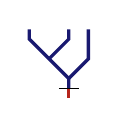
\begin{tikzpicture}[scale=0.25]
\draw[very thick, MidnightBlue] (0,-0.5)--(0,0) -- (-2,2)--(-2,2.5);
\draw[very thick, MidnightBlue] (-1,1)--(0,2)--(0,2.5) ;
\draw[very thick, MidnightBlue] (0,0)--(1,1)--(1,2.5) ;
%
\draw[very thick, BrickRed] (0,-0.5)--(0,-1) ;
%
\draw (-0.5,-0.5) --(0.5, -0.5);
\end{tikzpicture}}}}

\newcommand{\TreeLb}
{\vcenter{\hbox{

\begin{tikzpicture}[scale=0.25]
\draw[very thick, MidnightBlue] (-0.5,0.5)--(-2,2)--(-2,2.5);
\draw[very thick, MidnightBlue] (-1,1)--(0,2)--(0,2.5) ;
\draw[very thick, MidnightBlue] (0.5,0.5)--(1,1)--(1,2.5) ;
%
\draw[very thick, BrickRed] (0,0)--(0,-0.5) ;
\draw[very thick, BrickRed] (0,0)--(-0.5, 0.5) ;
\draw[very thick, BrickRed] (0,0)--(0.5,0.5) ;
%
\draw (-1,0.5) --(1, 0.5);
\end{tikzpicture}}}}

\newcommand{\TreeLc}
{\vcenter{\hbox{
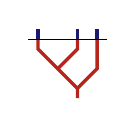
\begin{tikzpicture}[scale=0.25]
\draw[very thick, MidnightBlue] (-2, 2.5)--(-2, 3) ;
\draw[very thick, MidnightBlue] (0, 2.5)--(0, 3) ;
\draw[very thick, MidnightBlue] (1, 2.5)--(1, 3) ;
%
\draw[very thick, BrickRed] (0,-0.5)--(0,0) -- (-2,2)--(-2,2.5);
\draw[very thick, BrickRed] (-1,1)--(0,2)--(0,2.5) ;
\draw[very thick, BrickRed] (0,0)--(1,1)--(1,2.5) ;
%
\draw (-2.5,2.5) --(1.5, 2.5);
\end{tikzpicture}}}}

\newcommand{\TreeRa}
{\vcenter{\hbox{
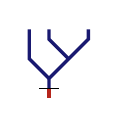
\begin{tikzpicture}[scale=0.25]
\draw[very thick, MidnightBlue] (0,-0.5)--(0,0) -- (2,2)--(2,2.5);
\draw[very thick, MidnightBlue] (1,1)--(0,2)--(0,2.5) ;
\draw[very thick, MidnightBlue] (0,0)--(-1,1)--(-1,2.5) ;
%
\draw[very thick, BrickRed] (0,-0.5)--(0,-1) ;
%
\draw (-0.5,-0.5) --(0.5, -0.5);
\end{tikzpicture}}}}

\newcommand{\TreeRb}
{\vcenter{\hbox{
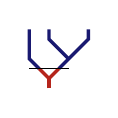
\begin{tikzpicture}[scale=0.25]
\draw[very thick, MidnightBlue] (0.5,0.5) -- (2,2)--(2,2.5);
\draw[very thick, MidnightBlue] (1,1)--(0,2)--(0,2.5) ;
\draw[very thick, MidnightBlue] (-0.5,0.5)--(-1,1)--(-1,2.5) ;
%
\draw[very thick, BrickRed] (0,-0.5)--(0,0) ;
\draw[very thick, BrickRed] (0,0)--(0.5,0.5) ;
\draw[very thick, BrickRed] (0,0)--(-0.5,0.5) ;
%
\draw (-1,0.5) --(1, 0.5);
\end{tikzpicture}}}}

\newcommand{\TreeRc}
{\vcenter{\hbox{
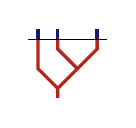
\begin{tikzpicture}[scale=0.25]
\draw[very thick, BrickRed] (0,-0.5)--(0,0) -- (2,2)--(2,2.5);
\draw[very thick, BrickRed] (1,1)--(0,2)--(0,2.5) ;
\draw[very thick, BrickRed] (0,0)--(-1,1)--(-1,2.5) ;
%
\draw[very thick, MidnightBlue] (2,2.5)--(2,3) ;
\draw[very thick, MidnightBlue] (0,2.5)--(0,3) ;
\draw[very thick, MidnightBlue] (-1,2.5)--(-1,3) ;
%
\draw (-1.5,2.5) --(2.5, 2.5);
\end{tikzpicture}}}}

\newcommand{\TreeLab}
{\vcenter{\hbox{
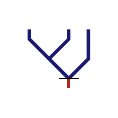
\begin{tikzpicture}[scale=0.25]
\draw[very thick, MidnightBlue] (0,0) -- (-2,2)--(-2,2.5);
\draw[very thick, MidnightBlue] (-1,1)--(0,2)--(0,2.5) ;
\draw[very thick, MidnightBlue] (0,0)--(1,1)--(1,2.5) ;
%
\draw[very thick, BrickRed] (0,0)--(0,-0.5) ;
%
\draw (-0.5,0) --(0.5, 0);
\end{tikzpicture}}}}

\newcommand{\TreeLbc}
{\vcenter{\hbox{
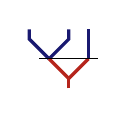
\begin{tikzpicture}[scale=0.25]
\draw[very thick, MidnightBlue] (-1,1) -- (-2,2)--(-2,2.5);
\draw[very thick, MidnightBlue] (-1,1)--(0,2)--(0,2.5) ;
\draw[very thick, MidnightBlue] (1,1)--(1,2.5) ;
%
\draw[very thick, BrickRed] (0,-0.5)--(0,0) ;
\draw[very thick, BrickRed] (0,0)--(-1,1) ;
\draw[very thick, BrickRed] (0,0)--(1,1) ;
%
\draw (-1.5,1) --(1.5, 1);
\end{tikzpicture}}}}

\newcommand{\TreeRab}
{\vcenter{\hbox{
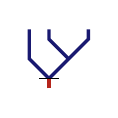
\begin{tikzpicture}[scale=0.25]
\draw[very thick, MidnightBlue] (0,0) -- (2,2)--(2,2.5);
\draw[very thick, MidnightBlue] (1,1)--(0,2)--(0,2.5) ;
\draw[very thick, MidnightBlue] (0,0)--(-1,1)--(-1,2.5) ;
%
\draw[very thick, BrickRed] (0,-0.5)--(0,0) ;
%
\draw (-0.5,0) --(0.5, 0);
\end{tikzpicture}}}}

\newcommand{\TreeRbc}
{\vcenter{\hbox{

\begin{tikzpicture}[scale=0.25]
\draw[very thick, MidnightBlue] (1,1) -- (2,2)--(2,2.5);
\draw[very thick, MidnightBlue] (1,1)--(0,2)--(0,2.5) ;
\draw[very thick, MidnightBlue] (-1,1)--(-1,2.5) ;
%
\draw[very thick, BrickRed] (0,-0.5)--(0,0) ;
\draw[very thick, BrickRed] (0,0)--(1,1) ;
\draw[very thick, BrickRed] (0,0)--(-1,1) ;
%
\draw (-1.5,1) --(1.5, 1);
\end{tikzpicture}}}}

\newcommand{\TreeCa}
{\vcenter{\hbox{
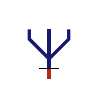
\begin{tikzpicture}[scale=0.25]
\draw[very thick, MidnightBlue] (0,-0.5) -- (0,1.5);
\draw[very thick, MidnightBlue] (0,0) -- (-1,1)--(-1,1.5);
\draw[very thick, MidnightBlue] (0,0) -- (1,1)--(1,1.5);
%
\draw[very thick, BrickRed] (0,-0.5)--(0,-1) ;
%
\draw (-0.5,-0.5) --(0.5, -0.5);
\end{tikzpicture}}}}

\newcommand{\TreeCb}
{\vcenter{\hbox{
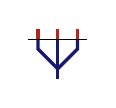
\begin{tikzpicture}[scale=0.25]
\draw[very thick, MidnightBlue] (0,-0.5) -- (0,1.5);
\draw[very thick, MidnightBlue] (0,0) -- (-1,1)--(-1,1.5);
\draw[very thick, MidnightBlue] (0,0) -- (1,1)--(1,1.5);
%
\draw[very thick, BrickRed] (-1,1.5)--(-1,2) ;
\draw[very thick, BrickRed] (0,1.5)--(0,2) ;
\draw[very thick, BrickRed] (1,1.5)--(1,2) ;
%
\draw (-1.5,1.5) --(1.5, 1.5);
\end{tikzpicture}}}}

\newcommand{\TreeCab}
{\vcenter{\hbox{

\begin{tikzpicture}[scale=0.25]
\draw[very thick, MidnightBlue] (0,0) -- (0,1.5);
\draw[very thick, MidnightBlue] (0,0) -- (-1,1)--(-1,1.5);
\draw[very thick, MidnightBlue] (0,0) -- (1,1)--(1,1.5);
%
\draw[very thick, BrickRed] (0,-0.5)--(0,0) ;
%
\draw (-0.5,0) --(0.5, 0);
\end{tikzpicture}}}}

\newcommand{\TreeIab}
{\vcenter{\hbox{
\begin{tikzpicture}[scale=0.35]
\draw[very thick, MidnightBlue] (0,0.5)--(0,0);
%
\draw[very thick, BrickRed] (0,-0.5)--(0,0) ;
%
\draw (-0.25,0) --(0.25, 0);
\end{tikzpicture}}}}

\newcommand{\TreeBa}
{\vcenter{\hbox{
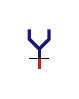
\begin{tikzpicture}[scale=0.25]
\draw[very thick, MidnightBlue] (0,0.5)--(0,1);
\draw[very thick, MidnightBlue] (0,1)--(-0.5,1.5)--(-0.5,2);
\draw[very thick, MidnightBlue] (0,1)--(0.5,1.5)--(0.5,2);
% 
\draw[very thick, BrickRed] (0,0)--(0,0.5);
\draw (-0.5,0.5) --(0.5, 0.5);\end{tikzpicture}}}}

\newcommand{\TreeBb}
{\vcenter{\hbox{
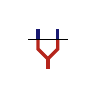
\begin{tikzpicture}[scale=0.25]
\draw[very thick, MidnightBlue] (-0.5,2)--(-0.5,2.5);
\draw[very thick, MidnightBlue] (0.5,2)--(0.5,2.5);
%
\draw[very thick, BrickRed] (0,0.5)--(0,1);
\draw[very thick, BrickRed] (0,1)--(-0.5,1.5)--(-0.5,2);
\draw[very thick, BrickRed] (0,1)--(0.5,1.5)--(0.5,2);
% 
\draw (-1,2) --(1, 2);
\end{tikzpicture}}}}

\newcommand{\TreeBab}
{\vcenter{\hbox{

\begin{tikzpicture}[scale=0.25]
\draw[very thick, MidnightBlue] (0,1)--(-0.5,1.5)--(-0.5,2);
\draw[very thick, MidnightBlue] (0,1)--(0.5,1.5)--(0.5,2);
% 
\draw[very thick, BrickRed] (0,0.5)--(0,1);
\draw (-0.5,1) --(0.5,1);
\end{tikzpicture}}}}

%%%% Trees OLD

\newcommand{\TreeR}
{\vcenter{\hbox{
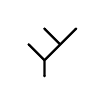
\begin{tikzpicture}[yscale=0.2,xscale=0.2]
\draw[thick] (0,-1)--(0,0) -- (2,2);
\draw[thick] (1,1)--(0,2) ;
\draw[thick] (0,0)--(-1,1) ;
\draw [fill] (0,-1) circle [radius=0.035];
\draw [fill] (2,2) circle [radius=0.035];
\draw [fill] (0,2) circle [radius=0.035];
\draw [fill] (-1,1) circle [radius=0.035];
\end{tikzpicture}}}}
\newcommand{\TreeL}
{\vcenter{\hbox{
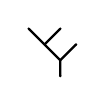
\begin{tikzpicture}[yscale=0.2,xscale=0.2]
\draw[thick] (0,-1)--(0,0) -- (-2,2);
\draw[thick] (-1,1)--(0,2) ;
\draw[thick] (0,0)--(1,1) ;
\draw [fill] (0,-1) circle [radius=0.035];
\draw [fill] (-2,2) circle [radius=0.035];
\draw [fill] (0,2) circle [radius=0.035];
\draw [fill] (1,1) circle [radius=0.035];
\end{tikzpicture}}}}
\newcommand{\TreeLL}
{\vcenter{\hbox{
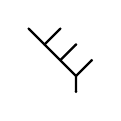
\begin{tikzpicture}[yscale=0.2,xscale=0.2]
\draw[thick] (0,-1)--(0,0) -- (-3,3);
\draw[thick] (-1,1)--(0,2) ;
\draw[thick] (-2,2)--(-1,3) ;
\draw[thick] (0,0)--(1,1) ;
\draw [fill] (0,-1) circle [radius=0.035];
\draw [fill] (-2,2) circle [radius=0.035];
\draw [fill] (0,2) circle [radius=0.035];
\draw [fill] (1,1) circle [radius=0.035];
\draw [fill] (-3,3) circle [radius=0.035];
\draw [fill] (-1,3) circle [radius=0.035];
\end{tikzpicture}}}}
\newcommand{\TreeLR}
{\vcenter{\hbox{
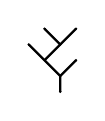
\begin{tikzpicture}[yscale=0.2,xscale=0.2]
\draw[thick] (0,-1)--(0,0) -- (-2,2);
\draw[thick] (-1,1)--(1,3) ;
\draw[thick] (0,0)--(1,1) ;
\draw[thick] (0,2)--(-1,3) ;
\draw [fill] (0,-1) circle [radius=0.035];
\draw [fill] (-2,2) circle [radius=0.035];
\draw [fill] (0,2) circle [radius=0.035];
\draw [fill] (1,1) circle [radius=0.035];
\draw [fill] (-1,3) circle [radius=0.035];
\draw [fill] (1,3) circle [radius=0.035];
\end{tikzpicture}}}}
\newcommand{\TreeRR}
{\vcenter{\hbox{
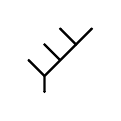
\begin{tikzpicture}[yscale=0.2,xscale=0.2]
\draw[thick] (0,-1)--(0,0) -- (3,3);
\draw[thick] (1,1)--(0,2) ;
\draw[thick] (2,2)--(1,3) ;
\draw[thick] (0,0)--(-1,1) ;
\draw [fill] (0,-1) circle [radius=0.035];
\draw [fill] (2,2) circle [radius=0.035];
\draw [fill] (0,2) circle [radius=0.035];
\draw [fill] (-1,1) circle [radius=0.035];
\draw [fill] (3,3) circle [radius=0.035];
\draw [fill] (1,3) circle [radius=0.035];
\end{tikzpicture}}}}
\newcommand{\TreeRL}
{\vcenter{\hbox{
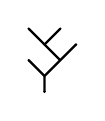
\begin{tikzpicture}[yscale=0.2,xscale=0.2]
\draw[thick] (0,-1)--(0,0) -- (2,2);
\draw[thick] (1,1)--(-1,3) ;
\draw[thick] (0,0)--(-1,1) ;
\draw[thick] (0,2)--(1,3) ;
\draw [fill] (0,-1) circle [radius=0.035];
\draw [fill] (2,2) circle [radius=0.035];
\draw [fill] (0,2) circle [radius=0.035];
\draw [fill] (-1,1) circle [radius=0.035];
\draw [fill] (1,3) circle [radius=0.035];
\draw [fill] (-1,3) circle [radius=0.035];
\end{tikzpicture}}}}
\newcommand{\TreeCC}
{\vcenter{\hbox{
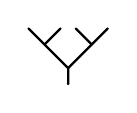
\begin{tikzpicture}[yscale=0.2,xscale=0.2]
\draw[thick] (0,-1)--(0,0) -- (-2.5,2.5);
\draw[thick] (-1.5,1.5)--(-0.5,2.5) ;
\draw[thick] (1.5,1.5)--(0.5,2.5) ;
\draw[thick] (0,0)--(2.5,2.5) ;
\draw [fill] (0,-1) circle [radius=0.035];
\draw [fill] (-2.5,2.5) circle [radius=0.035];
\draw [fill] (-0.5,2.5) circle [radius=0.035];
\draw [fill] (0.5,2.5) circle [radius=0.035];
\draw [fill] (2.5,2.5) circle [radius=0.035];
\end{tikzpicture}}}}
\newcommand{\TreeAL}
{\vcenter{\hbox{
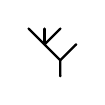
\begin{tikzpicture}[yscale=0.2,xscale=0.2]
\draw[thick] (0,-1)--(0,0) -- (-2,2);
\draw[thick] (-1,1)--(0,2) ;
\draw[thick] (0,0)--(1,1) ;
\draw[thick] (-1,1)--(-1,2) ;
\draw [fill] (0,-1) circle [radius=0.035];
\draw [fill] (-2,2) circle [radius=0.035];
\draw [fill] (0,2) circle [radius=0.035];
\draw [fill] (1,1) circle [radius=0.035];
\draw [fill] (-1,2) circle [radius=0.035];
\end{tikzpicture}}}}
\newcommand{\TreeRA}
{\vcenter{\hbox{
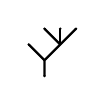
\begin{tikzpicture}[yscale=0.2,xscale=0.2]
\draw[thick] (0,-1)--(0,0) -- (2,2);
\draw[thick] (1,1)--(0,2) ;
\draw[thick] (0,0)--(-1,1) ;
\draw[thick] (1,1)--(1,2) ;
\draw [fill] (0,-1) circle [radius=0.035];
\draw [fill] (2,2) circle [radius=0.035];
\draw [fill] (0,2) circle [radius=0.035];
\draw [fill] (-1,1) circle [radius=0.035];
\draw [fill] (1,2) circle [radius=0.035];
\end{tikzpicture}}}}
\newcommand{\TreeAR}
{\vcenter{\hbox{
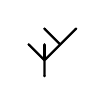
\begin{tikzpicture}[yscale=0.2,xscale=0.2]
\draw[thick] (0,-1)--(0,0) -- (2,2);
\draw[thick] (1,1)--(0,2) ;
\draw[thick] (0,0)--(-1,1) ;
\draw[thick] (0,0)--(0,1) ;
\draw [fill] (0,-1) circle [radius=0.035];
\draw [fill] (2,2) circle [radius=0.035];
\draw [fill] (0,2) circle [radius=0.035];
\draw [fill] (-1,1) circle [radius=0.035];
\draw [fill] (0,1) circle [radius=0.035];
\end{tikzpicture}}}}
\newcommand{\TreeLA}
{\vcenter{\hbox{
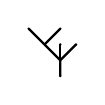
\begin{tikzpicture}[yscale=0.2,xscale=0.2]
\draw[thick] (0,-1)--(0,0) -- (-2,2);
\draw[thick] (-1,1)--(0,2) ;
\draw[thick] (0,0)--(1,1) ;
\draw[thick] (0,0)--(0,1) ;
\draw [fill] (0,-1) circle [radius=0.035];
\draw [fill] (-2,2) circle [radius=0.035];
\draw [fill] (0,2) circle [radius=0.035];
\draw [fill] (1,1) circle [radius=0.035];
\draw [fill] (0,1) circle [radius=0.035];
\end{tikzpicture}}}}
\newcommand{\TreeCA}
{\vcenter{\hbox{
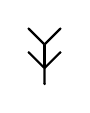
\begin{tikzpicture}[yscale=0.2,xscale=0.2]
\draw[thick] (0,-1)--(0,0) -- (-1,1);
\draw[thick] (0,1.5)--(1,2.5) ;
\draw[thick] (0,1.5)--(-1,2.5) ;
\draw[thick] (0,0)--(1,1) ;
\draw[thick] (0,0)--(0,1.5) ;
\draw [fill] (0,-1) circle [radius=0.035];
\draw [fill] (-1,1) circle [radius=0.035];
\draw [fill] (1,2.5) circle [radius=0.035];
\draw [fill] (-1,2.5) circle [radius=0.035];
\draw [fill] (1,1) circle [radius=0.035];
\draw [fill] (0,1) circle [radius=0.035];
\end{tikzpicture}}}}
\newcommand{\TreeC}
{\vcenter{\hbox{
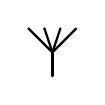
\begin{tikzpicture}[yscale=0.2,xscale=0.2]
\draw[thick] (0,-1.5)--(0,0);
\draw[thick] (0,0)--(1.5,1.5) ;
\draw[thick] (0,0)--(0.5,1.5) ;
\draw[thick] (0,0)--(-0.5,1.5) ;
\draw[thick] (0,0)--(-1.5,1.5) ;
\draw [fill] (0,-1.5) circle [radius=0.035];
\draw [fill] (1.5,1.5) circle [radius=0.035];
\draw [fill] (0.5,1.5) circle [radius=0.035];
\draw [fill] (-1.5,1.5) circle [radius=0.035];
\draw [fill] (-0.5,1.5) circle [radius=0.035];
\end{tikzpicture}}}}

%Drapeau européen

\usepackage{graphicx,calc}
\newlength\myheight
\newlength\mydepth
\settototalheight\myheight{Xygp}
\settodepth\mydepth{Xygp}
\setlength\fboxsep{0pt}
\newcommand*\inlinegraphics[1]{%
  \settototalheight\myheight{Xygp}%
  \settodepth\mydepth{Xygp}%
  \raisebox{-\mydepth}{\includegraphics[height=\myheight]{#1}}%
}

%%%%%%%%% Nouveau

\DeclareMathOperator{\Ima}{Im} %Image d'une fonction
\DeclareMathOperator{\cone}{Cone} %Cône

%%%%%%%%%%%   Comments 

\newcommand{\Thibaut}[1]{\textcolor{red}{#1}}
\newcommand{\Guillaume}[1]{\textcolor{blue}{#1}}

%%%%%% TITLE+AUTHOR

\title{The diagonal of the multiplihedra and the product of A-infinity categories}

\author{Guillaume Laplante-Anfossi}
\address{Laboratoire Analyse, G\'eom\'etrie et Applications, Universit\'e Paris Nord 13, Sorbonne Paris Cit\'e, CNRS, UMR 7539, 93430 Villetaneuse, France.}
\email{laplante-anfossi@math.univ-paris13.fr}

\author{Thibaut Mazuir}
\address{Sorbonne Universit\'e, Institut de Math\'ematiques de Jussieu-Paris Rive Gauche CNRS, Campus Pierre et Marie Curie, 75013 Paris, France.}
\email{thibaut.mazuir@imj-prg.fr}

\date{\today}

\subjclass[2010]{Primary 52B11; Secondary 18M70, 53D37}

\keywords{Multiplihedra, A-infinity categories, approximation of the diagonal, operads.}

\thanks{The first author was supported by the European Union's Horizon 2020 research and innovation program under the Marie Sklodowska-Curie grant agreement No 754362 \inlinegraphics{EU.png}, by the Natural Sciences and Engineering Research Council of Canada (NSERC) and by the ANR-20-CE40-0016 Higher Algebra, Geometry and Topology.}

\begin{document}

\begin{abstract}
The goal of this article is to define a cellular approximation to the diagonal of Forcey--Loday realizations of the multiplihedra, and to endow them with a compatible topological cellular operadic bimodule structure over the Loday realizations of the associahedra. 
This gives a model for topological and algebraic A-infinity morphisms, and an explicit formula for their tensor product.
In this way, one can consider for the first time a functorial tensor product of A-infinity categories defined by explicit formulas, and its potential applications, notably to Fukaya categories in symplectic topology. 
\end{abstract}

\maketitle

\begin{figure}[h!]
\centering
\includegraphics[width=0.7\linewidth]{J4.png} 
%\caption{The polytopal subdivision of $\J_4$.}
\label{Fig5:J4}
\end{figure}

\setcounter{tocdepth}{1}
\tableofcontents

%%%%%%%%%%%%%%%%%%%%%%%%%%%%%%%%%%%%%%%%

\section*{Introduction}

The $n$-dimensional associahedron, a polytope whose faces are in bijection with planar trees with $n+1$ leaves, was introduced as a topological cell complex by J. Stasheff to describe algebras whose product is associative only up to homotopy \cite{Stasheff63}.
The problem of giving convex realizations of these polytopes has a rich history \cite{CeballosZiegler12}, and the algebras that they encode, called $\mathrm{A}_\infty$-algebras, are now classical objects in algebraic topology. 
They have found many applications, from iterated loop spaces \cite{May72} to Fukaya categories \cite{Seidel08}, through the interpretation of the associahedra as moduli spaces of metric trees \cite{MauWoodward10}.

\medskip

The $n$-dimensional multiplihedron, a polytope whose faces are in bijection with 2-colored planar trees with $n$ leaves (see \cref{def:2coloredtree} below), was introduced by J. Stasheff \cite{Stasheff70} to describe morphisms between $\mathrm{A}_\infty$-algebras.
These polytopes were studied both in algebraic topology \cite{BoardmanVogt73} and symplectic topology, through their interpretation as moduli spaces of 2-colored metric trees \cite{MauWoodward10}. 
First defined as topological cell complexes, they were only realized recently as convex polytopes, through the work of S. Forcey \cite{Forcey08}, and later S. Forcey and S. Devadoss \cite{DevadossForcey08}, F. Ardila and J. Doker \cite{AD13}, and F. Chapoton and V. Pilaud \cite{CP22}.

\medskip

In this paper, we study a cellular approximation to the diagonal of the multiplihedron. 
The set-theoretic diagonal $\triangle_P:P\to P\times P, x\mapsto (x,x)$ of a polytope $P$ is not cellular, that is, its image is not a union of faces of $P\times P$. 
One is led to the problem of finding a cellular approximation to $\triangle_P$, that is finding a cellular map $\triangle_P^{\textrm{cell}} : P \to P\times P$ which is homotopic to $\triangle_P$ and which agrees with $\triangle_P$ on the vertices of $P$.

\medskip

The Alexander--Whitney map \cite{EilenbergMacLane53} and the Serre diagonal \cite{Serre51} are cellular approximations of the diagonal of the simplices and the cubes, respectively. 
They allow one to define the cup product in cohomology.
A cellular approximation of the diagonal of the associahedra allows one to define the tensor product of two $\mathrm{A}_\infty$-algebras \cite{SaneblidzeUmble04,MarklShnider06,MTTV19}. 
Our goal here is to make this tensor product functorial, by defining and describing explicitly a cellular approximation to the diagonal of the multiplihedra.

\medskip

Our results can be summarized as follows:
\begin{enumerate}
  \item We define a cellular approximation of the diagonal of the Forcey--Loday realizations of the multiplihedra (\cref{prop:OrientationVector});
  \item We endow them with a compatible topological cellular operadic bimodule structure over the Loday realizations of the associahedra (\cref{thm:MainOperad});
  \item We describe combinatorially the cellular image of the diagonal (\cref{thm:formuladiagonal});
  \item We apply the cellular chains functor to obtain a functorial tensor product of $\mathrm{A}_\infty$-algebras and their categorification, $\mathrm{A}_\infty$-categories.
\end{enumerate}


To achieve these goals, we use the general theory developed by the first author in \cite{LA21}, based on the method introduced in \cite{MTTV19}. 
More precisely, we use the fact that the Forcey--Loday realization of the multiplihedron, as defined in \cite{Forcey08}, can be obtained from the Ardila--Doker realization of the multiplihedron \cite{AD13} by projection.
This last realization is a generalized permutahedron, in the sense of A. Postnikov \cite{Postnikov09}, which allows us to apply the results of \cite{LA21} directly, both for the purpose of defining a cellular approximation of the diagonal, and to describe its cellular image combinatorially.

\medskip

Our results can readily be applied to different fields, prominently to symplectic topology. 
First, the operadic bimodule structure in~(2) above was used in the work of the second author, where the structures of $\mathrm{A}_\infty$-algebras and $\mathrm{A}_\infty$-morphisms are unraveled in the context of Morse theory \cite{Mazuir21}. 
Second, our definition of a functorial tensor product of $\mathrm{A}_\infty$-categories by explicit formulas can be used to study the Fukaya categories of symplectic manifolds. %deformations of bordered Riemann surfaces and the work of Liu
It could also be used in the context of bordered Heegaard Floer homology to compute invariants of 4-manifolds \cite{LOT20}. 
See \cref{sec:furtherdirections} where we sketch some applications to symplectic topology.
One could also think to applications in other areas where the multiplihedron appears, such as higher category theory \cite{ForceyQuotient08}.

\medskip

Finally, the methods of this paper can be straightfowardly extended to the "multiploperahedra", a family of polytopes which is to the operahedra of \cite{LA21} what the multiplihedra are to the associahedra. 
They belong to both the families of graph-multiplihedra \cite{DevadossForcey08} and nestomultiplihedra \cite{AD13}.  
Together with the results of \cite{LA21}, one would obtain a functorial tensor product of homotopy operads, defined by explicit formulas. 

\subsection*{Layout} 
We define the realizations of the multiplihedra we will work with in \cref{sec:I}. 
We define a cellular approximation of their diagonal and endow them with an operadic bimodule structure over the associahedra in \cref{sec:II}.
We describe explicitly the image of our diagonal combinatorially, define the functorial tensor product of $\mathrm{A}_\infty$-categories, and sketch applications to symplectic topology in \cref{sec:III}. 

\subsection*{Conventions} We use the conventions and notations of \cite{Ziegler95} for convex polytopes and the ones of \cite{LodayVallette12} for operads. We denote by $[n]\coloneqq \{1,\ldots,n\}$ and by $\{\vec e_i\}_{i \in [n]}$ the standard basis of $\RR^n$.

\subsection*{Acknowledgements} 
We would like to thank Bruno Vallette for numerous discussions and for his careful reading of the manuscript.
We are also indebted to Robert Lipshitz for his detailed insights about the possible applications of our results in symplectic topology.


%%%%%%%%%%%%%%%%%%%%%%%%%%%%%%%%%%%%%%%%%%%%

\section{Realization of the muliplihedra} 
\label{sec:I}

Building on the work of S. Forcey in \cite{Forcey08}, we define Forcey--Loday realizations of the multiplihedra, and describe their general properties in \cref{prop:PropertiesKLoday}.
We show how they can be obtained from the Ardila--Doker realizations via projection. 

%%%%%%%%%%%%%%%%%%%%%%%%%%%%%%%%%%%%%%%%%%%%%

\subsection{Colored trees}

We consider planar rooted trees, which we will abbreviate simply trees. The term "edge" refers to both internal and external edges. The external edges we will sometimes call leaves. 

\begin{definition}[Cut]
A \emph{cut} of a tree is a subset of edges or vertices which contains precisely one edge or vertex along the unique path from the root to any leaf.
\end{definition}

A cut divides a tree into two parts: an upper part, that we color in blue, and a lower part, that we color in red.  

\begin{definition}[2-colored tree] \label{def:2coloredtree}
A \emph{2-colored tree} is a tree together with a cut. We call \emph{2-colored maximal tree} a 2-colored binary tree where the cut is made of edges only. 
\end{definition}
We denote by $\CT{n}$ (resp. $\CMT{n}$) the set of 2-colored trees (resp. 2-colored maximal trees) with $n$ leaves, for $n\geq 1$. 

\begin{figure}[h]
\[\vcenter{\hbox{
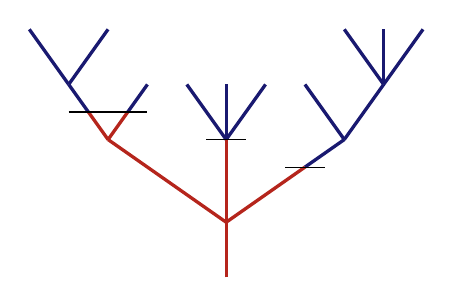
\begin{tikzpicture}[yscale=0.7,xscale=1]
%\draw[help lines] (-3,-1) grid (4,3);
%TOP
\draw[very thick, MidnightBlue] (-2.5,3.5)--(-2,2.5);
\draw[very thick, MidnightBlue] (-1.5,3.5)--(-2,2.5);
\draw[very thick, MidnightBlue] (-2,2.5) -- (-1.75,2);
\draw[very thick, MidnightBlue] (-1.25, 2) -- (-1,2.5);
\draw[very thick, MidnightBlue] (-0.5,2.5) -- (0,1.5);
\draw[very thick, MidnightBlue] (0,1.5)--(0,2.5);
\draw[very thick, MidnightBlue] (0,1.5)--(0.5,2.5);
\draw[very thick, MidnightBlue] (1,1)--(1.5,1.5);
\draw[very thick, MidnightBlue] (1.5,1.5)--(1,2.5);
\draw[very thick, MidnightBlue] (1.5,1.5)--(2,2.5);
\draw[very thick, MidnightBlue] (2,2.5)--(1.5,3.5);
\draw[very thick, MidnightBlue] (2,2.5)--(2,3.5);
\draw[very thick, MidnightBlue] (2,2.5)--(2.5,3.5);
%BOT
\draw[very thick, BrickRed] (0,-1)--(0, 1.5); 
\draw[very thick, BrickRed] (0,0)--(-1.5,1.5);
\draw[very thick, BrickRed] (-1.5,1.5)--(-1.75, 2); 
\draw[very thick, BrickRed] (-1.5,1.5)--(-1.25, 2); 
\draw[very thick, BrickRed] (0,0)--(1, 1);
% Frontier
\draw (-2,2) to (-1,2); 
\draw (-0.25,1.5)-- (0.25, 1.5) ; 
\draw (0.75,1) to (1.25,1);
\end{tikzpicture}}}\]
\caption{An example of a 2-colored tree.}
\label{Fig1:2ColTree}
\end{figure}

\begin{definition}[Face order and Tamari-type order]\leavevmode

\begin{itemize}
\item[$\diamond$] 
The \emph{face order} $s\subset t$ on 2-colored trees is defined as follows: a 2-colored tree $s$ is less than a 2-colored tree $t$ if $t$ can be obtained from $s$ by a sequence of contractions of monochrome edges or moves of the color frontier from an edge to an adjacent vertex.

\begin{figure}[h]
\[\vcenter{\hbox{
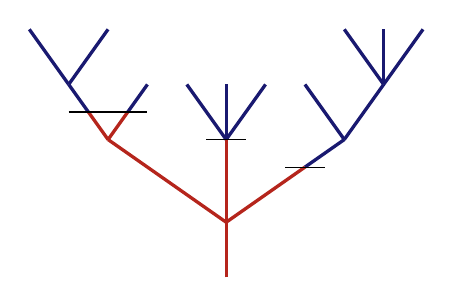
\begin{tikzpicture}[yscale=0.7,xscale=1]
%TOP
\draw[very thick, MidnightBlue] (-2.5,3.5)--(-2,2.5);
\draw[very thick, MidnightBlue] (-1.5,3.5)--(-2,2.5);
\draw[very thick, MidnightBlue] (-2,2.5) -- (-1.75,2);
\draw[very thick, MidnightBlue] (-1.25, 2) -- (-1,2.5);
\draw[very thick, MidnightBlue] (-0.5,2.5) -- (0,1.5);
\draw[very thick, MidnightBlue] (0,1.5)--(0,2.5);
\draw[very thick, MidnightBlue] (0,1.5)--(0.5,2.5);
\draw[very thick, MidnightBlue] (1,1)--(1.5,1.5);
\draw[very thick, MidnightBlue] (1.5,1.5)--(1,2.5);
\draw[very thick, MidnightBlue] (1.5,1.5)--(2,2.5);
\draw[very thick, MidnightBlue] (2,2.5)--(1.5,3.5);
\draw[very thick, MidnightBlue] (2,2.5)--(2,3.5);
\draw[very thick, MidnightBlue] (2,2.5)--(2.5,3.5);
%BOT
\draw[very thick, BrickRed] (0,-1)--(0, 1.5); 
\draw[very thick, BrickRed] (0,0)--(-1.5,1.5);
\draw[very thick, BrickRed] (-1.5,1.5)--(-1.75, 2); 
\draw[very thick, BrickRed] (-1.5,1.5)--(-1.25, 2); 
\draw[very thick, BrickRed] (0,0)--(1, 1);
% Frontier
\draw (-2,2) to (-1,2); 
\draw (-0.25,1.5)-- (0.25, 1.5) ; 
\draw (0.75,1) to (1.25,1);
\end{tikzpicture}}}
\quad \subset \quad
\vcenter{\hbox{
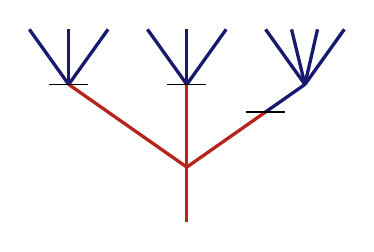
\begin{tikzpicture}[yscale=0.7,xscale=1]
%TOP
\draw[very thick, MidnightBlue] (-1.5,1.5)--(-1.5,2.5);
\draw[very thick, MidnightBlue] (-2,2.5) -- (-1.75,2);
\draw[very thick, MidnightBlue] (-1.25, 2) -- (-1,2.5);
\draw[very thick, MidnightBlue] (-0.5,2.5) -- (0,1.5);
\draw[very thick, MidnightBlue] (0,1.5)--(0,2.5);
\draw[very thick, MidnightBlue] (0,1.5)--(0.5,2.5);
\draw[very thick, MidnightBlue] (1,1)--(1.5,1.5);
\draw[very thick, MidnightBlue] (1.5,1.5)--(1,2.5);
\draw[very thick, MidnightBlue] (1.5,1.5)--(1.33,2.5);
\draw[very thick, MidnightBlue] (1.5,1.5)--(1.66,2.5);
\draw[very thick, MidnightBlue] (1.5,1.5)--(2,2.5);
\draw[very thick, MidnightBlue] (-1.5,1.5)--(-1.75, 2); 
\draw[very thick, MidnightBlue] (-1.5,1.5)--(-1.25, 2); 
%BOT
\draw[very thick, BrickRed] (0,-1)--(0, 1.5); 
\draw[very thick, BrickRed] (0,0)--(-1.5,1.5);
\draw[very thick, BrickRed] (0,0)--(1, 1);
% Frontier
\draw (-1.75,1.5) to (-1.25,1.5); 
\draw (-0.25,1.5) to (0.25,1.5); 
\draw (0.75,1) to (1.25,1);
\end{tikzpicture}}}
\]
\caption{An example of the face order $s\subset t$.}
\label{Fig2:InclusionOrder}
\end{figure}

\item[$\diamond$] The \emph{Tamari-type order} $s<t$ on  2-colored maximal trees is generated by the following three  covering relations: 
\[
{\vcenter{\hbox{
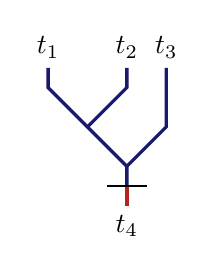
\begin{tikzpicture}[yscale=0.5,xscale=0.5]
\draw[very thick, MidnightBlue] (0,-0.5)--(0,0) -- (-2,2)--(-2,2.5);
\draw[very thick, MidnightBlue] (-1,1)--(0,2)--(0,2.5) ;
\draw[very thick, MidnightBlue] (0,0)--(1,1)--(1,2.5) ;
%
\draw[very thick, BrickRed] (0,-0.5)--(0,-1) ;
%
\draw (-0.5,-0.5) --(0.5, -0.5);
%
\draw (-2,2.5) node[above] {$t_1$}; 
\draw (0,2.5) node[above] {$t_2$}; 
\draw (1,2.5) node[above] {$t_3$}; 
\draw (0,-1) node[below] {$t_4$}; 
\end{tikzpicture}}}}
\prec
{\vcenter{\hbox{
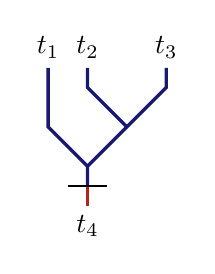
\begin{tikzpicture}[yscale=0.5,xscale=0.5]
\draw[very thick, MidnightBlue] (0,-0.5)--(0,0) -- (2,2)--(2,2.5);
\draw[very thick, MidnightBlue] (1,1)--(0,2)--(0,2.5) ;
\draw[very thick, MidnightBlue] (0,0)--(-1,1)--(-1,2.5) ;
%
\draw[very thick, BrickRed] (0,-0.5)--(0,-1) ;
%
\draw (-0.5,-0.5) --(0.5, -0.5);
%
\draw (2,2.5) node[above] {$t_3$}; 
\draw (0,2.5) node[above] {$t_2$}; 
\draw (-1,2.5) node[above] {$t_1$}; 
\draw (0,-1) node[below] {$t_4$}; 
\end{tikzpicture}}}}\ , \quad 
{\vcenter{\hbox{
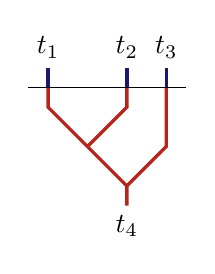
\begin{tikzpicture}[yscale=0.5,xscale=0.5]
\draw[very thick, MidnightBlue] (-2, 2.5)--(-2, 3) ;
\draw[very thick, MidnightBlue] (0, 2.5)--(0, 3) ;
\draw[very thick, MidnightBlue] (1, 2.5)--(1, 3) ;
%
\draw[very thick, BrickRed] (0,-0.5)--(0,0) -- (-2,2)--(-2,2.5);
\draw[very thick, BrickRed] (-1,1)--(0,2)--(0,2.5) ;
\draw[very thick, BrickRed] (0,0)--(1,1)--(1,2.5) ;
%
\draw (-2.5,2.5) --(1.5, 2.5);
%
\draw (-2,3) node[above] {$t_1$}; 
\draw (0,3) node[above] {$t_2$}; 
\draw (1,3) node[above] {$t_3$}; 
\draw (0,-0.5) node[below] {$t_4$}; 
\end{tikzpicture}}}}
\prec
{\vcenter{\hbox{
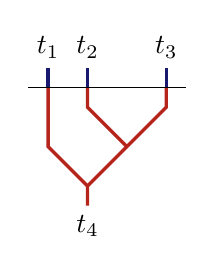
\begin{tikzpicture}[yscale=0.5,xscale=0.5]
\draw[very thick, BrickRed] (0,-0.5)--(0,0) -- (2,2)--(2,2.5);
\draw[very thick, BrickRed] (1,1)--(0,2)--(0,2.5) ;
\draw[very thick, BrickRed] (0,0)--(-1,1)--(-1,2.5) ;
%
\draw[very thick, MidnightBlue] (2,2.5)--(2,3) ;
\draw[very thick, MidnightBlue] (0,2.5)--(0,3) ;
\draw[very thick, MidnightBlue] (-1,2.5)--(-1,3) ;
%
\draw (-1.5,2.5) --(2.5, 2.5);
%
\draw (2,3) node[above] {$t_3$}; 
\draw (0,3) node[above] {$t_2$}; 
\draw (-1,3) node[above] {$t_1$}; 
\draw (0,-0.5) node[below] {$t_4$}; 
\end{tikzpicture}}}}\ , \quad 
{\vcenter{\hbox{
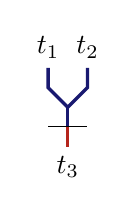
\begin{tikzpicture}[yscale=0.5,xscale=0.5]
\draw[very thick, MidnightBlue] (0,0.5)--(0,1);
\draw[very thick, MidnightBlue] (0,1)--(-0.5,1.5)--(-0.5,2);
\draw[very thick, MidnightBlue] (0,1)--(0.5,1.5)--(0.5,2);
% 
\draw[very thick, BrickRed] (0,0)--(0,0.5);
\draw (-0.5,0.5) --(0.5, 0.5);
%
\draw (-0.5,2) node[above] {$t_1$}; 
\draw (0.5,2) node[above] {$t_2$}; 
\draw (0,0) node[below] {$t_3$}; 
\end{tikzpicture}}}}
\prec
{\vcenter{\hbox{
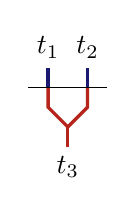
\begin{tikzpicture}[yscale=0.5,xscale=0.5]
\draw[very thick, MidnightBlue] (-0.5,2)--(-0.5,2.5);
\draw[very thick, MidnightBlue] (0.5,2)--(0.5,2.5);
%
\draw[very thick, BrickRed] (0,0.5)--(0,1);
\draw[very thick, BrickRed] (0,1)--(-0.5,1.5)--(-0.5,2);
\draw[very thick, BrickRed] (0,1)--(0.5,1.5)--(0.5,2);
% 
\draw (-1,2) --(1, 2);
%
\draw (-0.5,2.5) node[above] {$t_1$}; 
\draw (0.5,2.5) node[above] {$t_2$}; 
\draw (0,0.5) node[below] {$t_3$}; 
\end{tikzpicture}}}}
\ ,\]
where $t_i$, for $1\leq i\leq 4$, are 2-colored maximal trees, of respective colors each time. 
\end{itemize}
\end{definition}

\begin{figure}[h]
\[\vcenter{\hbox{
\begin{tikzcd}[column sep=0.5cm, row sep=0.5cm]
& \TreeLa \arrow[ld, thin] \arrow[rr, thin]&& \TreeRa \arrow[rd, thin]& \\
\TreeLb \arrow[rd, thin] &&&& \TreeRb \arrow[ld, thin] \\
& \TreeLc \arrow[rr, thin] && \TreeRc &
\end{tikzcd}
}}\]
\caption{The Tamari-type poset $(\CMT{3}, <)$ with minimum at the top.}
\label{Fig3:Tam}
\end{figure}

We often add a minimum element $\emptyset_n$ to the poset of 2-colored trees. 

\begin{proposition}
The posets $(\CT{n}, \subset)$ and $(\CMT{n}, <)$ are lattices. 
\end{proposition}

\begin{proof}
The poset of 2-colored trees was proven in \cite{Forcey08} to be isomorphic to the face lattice of a polytope, the multiplihedron; see Point~(3) of \cref{prop:PropertiesKLoday}. 
The Hasse diagram of the poset of 2-colored maximal trees was proven to be isomorphic to the oriented 1-skeleton of the multiplihedron, and also to be the Hasse diagram of a lattice in \cite[Proposition 117]{CP22}.
\end{proof}

\begin{remark}
V. Pilaud and F. Chapoton introduced in \cite{CP22} the shuffle of two generalized permutahedra, which is again a generalized permutahedron (see \cref{sec:generalizedpermutahedra} for definition and examples).
The fact that the poset $(\CMT{n}, <)$ is a lattice follows from the fact that the multiplihedron arises as the shuffle of the associahedron and the interval, which both have the lattice property, and that the shuffle operation preserves the lattice property in this case \cite[Corollary 95]{CP22}. 
However, the shuffle operation does not preserve the lattice property in general, see \cite[Remark~140]{CP22}.  
\end{remark}

%%%%%%%%%%%%%%%%%%%%%%%%%%%%%%%%%%%%%%%%%%%%%

\subsection{Multiplihedra} \label{sec:multiplihedra}

\begin{definition}[Multiplihedra]
For any $n\geq 1$, an \emph{$(n-1)$-dimensional multiplihedron} is a polytope whose face lattice is isomorphic to the lattice 
$(\CT{n}, \subset)$
of 2-colored trees with $n$ leaves. 
\end{definition}

\begin{figure}[h]
\[
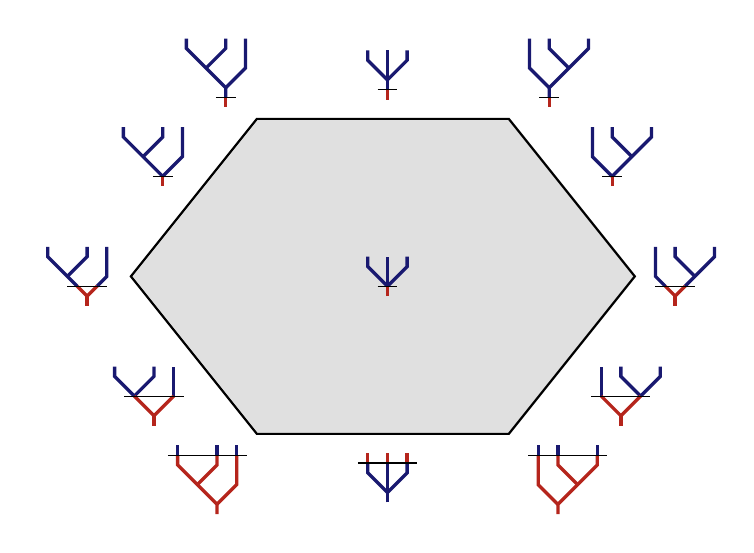
\begin{tikzpicture}[xscale=0.8,yscale=1]
\draw[thick] (-2,2)--(2,2)--(4,0)--(2,-2)--(-2,-2)--(-4,0)--cycle;
\draw[fill, opacity=0.12] (-2,2)--(2,2)--(4,0)--(2,-2)--(-2,-2)--(-4,0)--cycle;
\draw (-2,2) node[above left] {$\TreeLa$};
\draw (2,2) node[above right] {$\TreeRa$};
\draw (-2,-2) node[below left] {$\TreeLc$};
\draw (2,-2) node[below right] {$\TreeRc$};
\draw (-4.2,0) node[left] {$\TreeLb$};
\draw (4,0) node[right] {$\TreeRb$};
\draw (-3,1) node[above left] {$\TreeLab$};
\draw (-3,-1) node[below left] {$\TreeLbc$};
\draw (3,1) node[above right] {$\TreeRab$};
\draw (3,-1) node[below right] {$\TreeRbc$};
\draw (0,2.1) node[above] {$\TreeCa$};
\draw (0,-2.1) node[below] {$\TreeCb$};
\draw (0,0) node  {$\TreeCab$};
\end{tikzpicture}
\]
\caption{A 2-dimensional multiplihedron.}
\label{Fig4:J3}
\end{figure}

The dimension of a face labeled by a 2-colored tree is given by the sum of the degrees of its vertices defined by 
\[
\left|{\vcenter{\hbox{
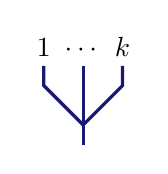
\begin{tikzpicture}[scale=0.5]
\draw[very thick, MidnightBlue] (0,-0.5) -- (0,1.5);
\draw[very thick, MidnightBlue] (0,0) -- (-1,1)--(-1,1.5);
\draw[very thick, MidnightBlue] (0,0) -- (1,1)--(1,1.5);
\draw (1,1.5) node[above] {$k$};
\draw (-1,1.5) node[above] {$1$};
\draw (0,1.5) node[above] {$\cdots$};
\end{tikzpicture}}}}\right|=k-2\ , \quad 
\left|{\vcenter{\hbox{
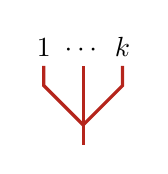
\begin{tikzpicture}[scale=0.5]
\draw[very thick, BrickRed] (0,-0.5) -- (0,1.5);
\draw[very thick, BrickRed] (0,0) -- (-1,1)--(-1,1.5);
\draw[very thick, BrickRed] (0,0) -- (1,1)--(1,1.5);
\draw (1,1.5) node[above] {$k$};
\draw (-1,1.5) node[above] {$1$};
\draw (0,1.5) node[above] {$\cdots$};
\end{tikzpicture}}}}\right|=k-2\ , \quad 
\left|{\vcenter{\hbox{
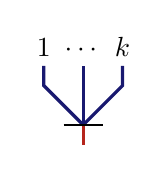
\begin{tikzpicture}[scale=0.5]
\draw[very thick, MidnightBlue] (0,0) -- (0,1.5);
\draw[very thick, MidnightBlue] (0,0) -- (-1,1)--(-1,1.5);
\draw[very thick, MidnightBlue] (0,0) -- (1,1)--(1,1.5);
\draw[very thick, BrickRed] (0,0) -- (0,-0.5);
\draw (-0.5,0)--(0.5,0);
\draw (1,1.5) node[above] {$k$};
\draw (-1,1.5) node[above] {$1$};
\draw (0,1.5) node[above] {$\cdots$};
\end{tikzpicture}}}}\right|=k-1\ .
\]
The codimension of a 2-colored tree is equal to the number of vertices of pure color. 
In the example of the 2-colored tree depicted on \cref{Fig1:2ColTree}, the dimension is equal to 4 and the codimension is equal to 5. 
As proven in \cite[Proposition 117]{CP22}, the oriented $1$-skeleton of a multiplihedron is the Hasse diagram of the Tamari-type poset. 

\medskip

Recall, for instance from \cite{MTTV19}, that one can also consider the set $\PT{n}$ of planar trees and the set $\Tam{n}$ of planar binary trees, with $n$ leaves. 
They are equipped with similar orders and an $(n-2)$-dimensional polytope whose face lattice agrees with the lattice $(\PT{n}, \subset)$  of planar trees is called an \emph{associahedron}. 
The grafting of trees endows planar (binary) trees with a non-symmetric operad structure and 2-colored (maximal) trees with an operadic bimodule structure over it. 
Regarding the right action, we denote the operation of grafting a planar tree $v$ at the $i^{\rm th}$-leaf of a 2-colored tree $u$ by $u\circ_i v$. 
Regarding the left action, we denote the grafting of a level of 2-colored trees $v_1, \ldots, v_k$ on the $k$ leaves of a planar tree by $u(v_1, \ldots, v_k)$. 
We denote by $c^{\T}_n$ and by $c^{\B}_n$ the corollas with $n$ leaves fully painted with the upper and the lower color respectively; we denote by $c_n$ the corolla with $n$ leaves with frontier color at the vertex. 
It is straightforward to see that these two grafting operations on corollas generate all the 2-colored trees of codimension $1$: we call $(\B)$, for ``bottom'', the first type of 2-colored trees $c_{p+1+r}\circ_{p+1} c^\T_q$, with $p+q+r=n$ and $2\leq q\leq n$, and we call  $(\T)$, for ``top'', the second type of 2-colored trees $c^\B_k(c_1, \ldots, c_k)$, with $i_1+\cdots+i_k=n$, $i_1, \ldots,i_k\geq 1$, and $k\geq 2$.

\begin{figure}[h]
\[\vcenter{\hbox{
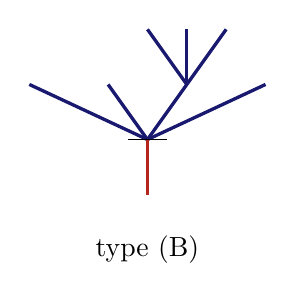
\begin{tikzpicture}[yscale=0.7,xscale=1]
%TOP
\draw[very thick, MidnightBlue] (0.5,1)--(0,2);
\draw[very thick, MidnightBlue] (0.5,1)--(0.5,2);
\draw[very thick, MidnightBlue] (0.5,1)--(1,2);
\draw[very thick, MidnightBlue] (0,0)--(0.5, 1); 
\draw[very thick, MidnightBlue] (0,0)--(-0.5, 1); 
\draw[very thick, MidnightBlue] (0,0)--(-1.5,1);
\draw[very thick, MidnightBlue] (0,0)--(1.5, 1);
%BOT
\draw[very thick, BrickRed] (0,-1)--(0, 0); 
% Frontier
\draw (-0.25,0) to (0.25,0); 
\draw (0,-2) node {type $(\B)$};
\end{tikzpicture}}}\qquad \vcenter{\hbox{
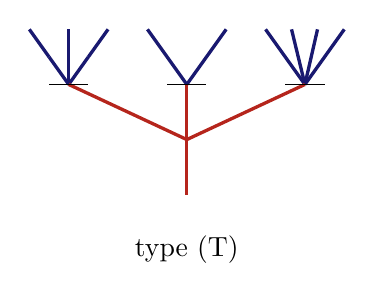
\begin{tikzpicture}[yscale=0.7,xscale=1]
%TOP
\draw[very thick, MidnightBlue] (-1.5,1)--(-1.5,2);
\draw[very thick, MidnightBlue] (-2,2) -- (-1.75,1.5);
\draw[very thick, MidnightBlue] (-1.25, 1.5) -- (-1,2);
\draw[very thick, MidnightBlue] (-0.5,2) -- (0,1);
\draw[very thick, MidnightBlue] (0,1)--(0.5,2);
\draw[very thick, MidnightBlue] (1.5,1)--(1,2);
\draw[very thick, MidnightBlue] (1.5,1)--(1.33,2);
\draw[very thick, MidnightBlue] (1.5,1)--(1.66,2);
\draw[very thick, MidnightBlue] (1.5,1)--(2,2);
\draw[very thick, MidnightBlue] (-1.5,1)--(-1.75, 1.5); 
\draw[very thick, MidnightBlue] (-1.5,1)--(-1.25, 1.5); 
%BOT
\draw[very thick, BrickRed] (0,-1)--(0, 1); 
\draw[very thick, BrickRed] (0,0)--(-1.5,1);
\draw[very thick, BrickRed] (0,0)--(1.5, 1);
% Frontier
\draw (-1.75,1) to (-1.25,1); 
\draw (-0.25,1) to (0.25,1); 
\draw (1.25,1) to (1.75,1);
\draw (0,-2) node {type $(\T)$};
\end{tikzpicture}}}\]
\caption{Examples of 2-colored trees of type $(\B)$ and $(\T)$ respectively. }
\label{Fig5:FacetsColoredTrees}
\end{figure}

%%%%%%%%%%%%%%%%%%%%%%%%%%%%%%%%%%%%%%%%%%%%

\subsection{Forcey--Loday realizations of the multiplihedra}
Jean-Louis Loday gave in \cite{Loday04a} realizations of the associahedra in the form of polytopes with integer coordinates. 
Stefan Forcey generalized this construction in \cite{Forcey08} in order to give similar realizations for the multiplihedra. 

\begin{definition}[Weighted 2-colored maximal tree]
A \emph{weighted 2-colored maximal tree} is a pair $(t, \omega)$ made up of a 2-colored maximal tree $t\in \CMT{n}$ with $n$ leaves with some weight $\omega= (\omega_1, \ldots, \omega_n) \in \RR_{>0}^n$. 
We call $\omega$ the \emph{weight} and
$n$ the \emph{arity} of the tree $t$ or the \emph{length} of the weight $\omega$.
\end{definition}

Let $(t, \omega)$ be a weighted 2-colored maximal tree with $n$ leaves. We order its $n-1$ vertices from left to right. At the $i^{\rm th}$ vertex, we consider the sum $\alpha_i$ of the weights of the leaves supported by its left input and 
 the sum $\beta_i$ of the weights of the leaves supported by its right input. 
If the $i^{\rm th}$ vertex is colored by the upper color, we consider the product $\alpha_i\beta_i$ and if the 
$i^{\rm th}$ vertex is colored by the lower color, we consider the product $2\alpha_i\beta_i$.
The associated string produces a point with integer coordinates :
\[M(t, \omega) \coloneqq \big(2\alpha_1\beta_1, \alpha_2\beta_2, \ldots, 2\alpha_{n-1}\beta_{n-1}\big)\in 
\RR_{>0}^{n-1}\ . \]
\begin{figure}[h!]
\[
\vcenter{\hbox{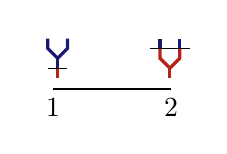
\begin{tikzpicture}[scale=1.5]
\draw[thick] (1,0)--(2,0);
\draw (1,0) node[above] {$\TreeBa$};
\draw (1.95,0) node[above] {$\TreeBb$};
\draw (1,0) node[below] {$1$};
\draw (2,0) node[below] {$2$};
\end{tikzpicture}}} \qquad \qquad
\vcenter{\hbox{
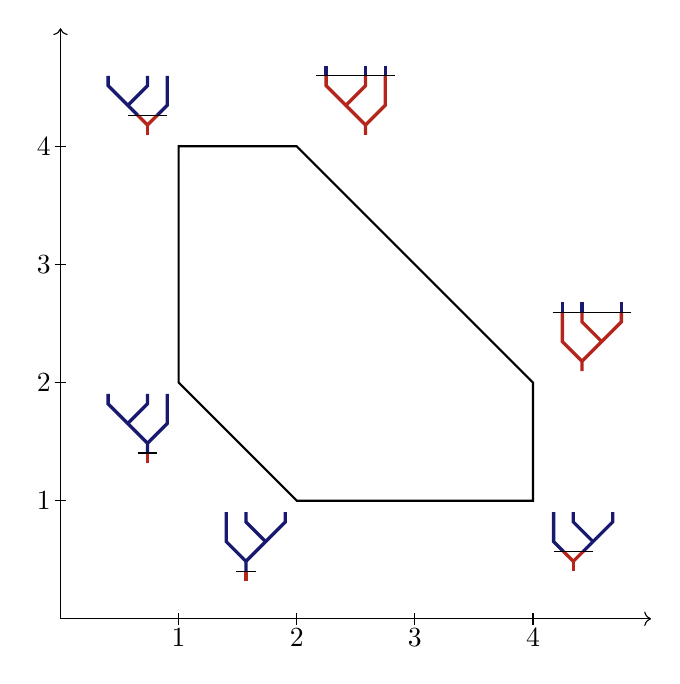
\begin{tikzpicture}[scale=1.5]
\draw (1,-0.05)--(1,0.05);
\draw (2,-0.05)--(2,0.05);
\draw (3,-0.05)--(3,0.05);
\draw (4,-0.05)--(4,0.05);
\draw (-0.05, 1)--(0.05,1);
\draw (-0.05, 2)--(0.05,2);
\draw (-0.05, 3)--(0.05,3);
\draw (-0.05, 4)--(0.05,4);
\draw[->] (0,0)--(5,0);
\draw[->] (0,0)--(0,5);
\draw (1,0) node[below] {$1$};
\draw (2,0) node[below] {$2$};
\draw (3,0) node[below] {$3$};
\draw (4,0) node[below] {$4$};
\draw (0,1) node[left] {$1$};
\draw (0,2) node[left] {$2$};
\draw (0,3) node[left] {$3$};
\draw (0,4) node[left] {$4$};
\draw[thick] (1,2)--(1,4)--(2,4)--(4,2)--(4,1)--(2,1)--cycle;
\draw (1,2) node[below left] {$\TreeLa$};
\draw (2,1) node[below left] {$\TreeRa$};
\draw (2,4) node[above right] {$\TreeLc$};
\draw (4,2) node[above right] {$\TreeRc$};
\draw (1,4) node[above left] {$\TreeLb$};
\draw (4,1) node[below right] {$\TreeRb$};
\end{tikzpicture}}}
\]
\caption{Examples of points associated to 2-colored maximal trees, with trivial weight.}
\end{figure}


\begin{definition}[Forcey--Loday Realization] \label{def:ForceyLoday}
 The \emph{Forcey--Loday realization of weight $\omega$} is the  polytope
\[\J_\omega \coloneqq \conv \big\{M(t, \omega)\mid t\in \CMT{n} \big\}\subset \RR^{n-1}\ .\]
\end{definition}

The Forcey--Loday realization associated to the standard weight $(1, \ldots, 1)$ is simply denoted by $\J_n$.
By convention, we define the polytope $\J_\omega$, with weight $\omega=(\omega_1)$ of length $1$,  to be made up of one point labeled by the 2-colored  tree $\iBT\coloneq \TreeIab$\ .
\begin{figure}[h]
\[
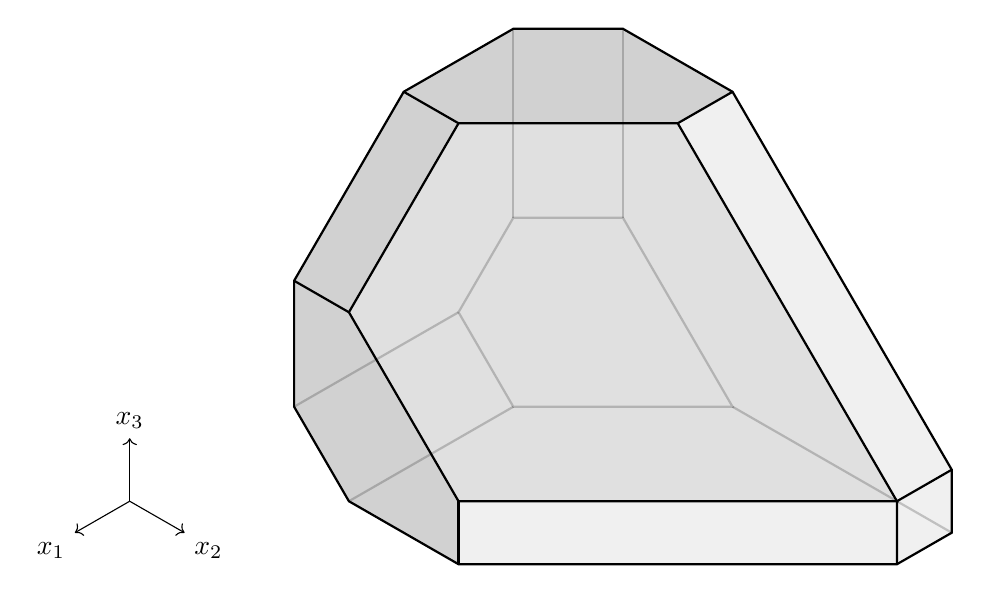
\begin{tikzpicture}[scale=0.8, J4]
\draw[->] (4,-4,-3)--(5,-4,-3) node[below left] {$x_1$};
\draw[->] (4,-4,-3)--(4,-3, -3) node[below right] {$x_2$};
\draw[->] (4,-4,-3)--(4,-4,-2) node[above] {$x_3$};

\draw[thick, opacity=0.2] (1,4,1)--(1,2,3)--(2,1,3)--(3,1,2)--(3,2,1)--cycle;
\draw[thick] (2,8,2)--(2,4,6)--(4,2,6)--(6,2,4)--(6,4,2)--cycle;
\draw[thick] (4,1,6)--(6,1,4)--(6,1,2)--(6,2,1)--(6,4,1)--(2,8,1)--(1,8,1)--(1,8,2)--(1,4,6)--(1,2,6)--(2,1,6)--cycle;
\draw[thick] (4,1,6)--(4,2,6);
\draw[thick] (6,1,4)--(6,2,4);
\draw[thick, opacity=0.2] (6,1,2)--(3,1,2);
\draw[thick, opacity=0.2] (6,2,1)--(3,2,1);
\draw[thick] (6,4,1)--(6,4,2);
\draw[thick] (2,8,1)--(2,8,2)--(1,8,2);
\draw[thick, opacity=0.2] (1,8,1)--(1,4,1);
\draw[thick] (1,4,6)--(2,4,6);
\draw[thick, opacity=0.2] (1,2,6)--(1,2,3);
\draw[thick, opacity=0.2] (2,1,6)--(2,1,3);

\draw[fill, opacity=0.12] (2,8,2)--(2,4,6)--(4,2,6)--(6,2,4)--(6,4,2)--cycle;
\draw[fill, opacity=0.18] (6,2,4)--(6,1,4)--(6,1,2)--(6,2,1)--(6,4,1)--(6,4,2)--cycle;
\draw[fill, opacity=0.18] (6,2,4)--(6,1,4)--(4,1,6)--(4,2,6)--cycle;
\draw[fill, opacity=0.18] (4,1,6)--(4,2,6)--(2,4,6)--(1,4,6)--(1,2,6)--(2,1,6)--cycle;
\draw[fill, opacity=0.06] (2,8,2)--(6,4,2)--(6,4,1)--(2,8,1)--cycle;
\draw[fill, opacity=0.06] (2,8,1)--(2,8,2)--(1,8,2)--(1,8,1)--cycle;
\draw[fill, opacity=0.06] (2,8,2)--(1,8,2)--(1,4,6)--(2,4,6)--cycle;
\end{tikzpicture}
\]
\caption{The Forcey--Loday realization of the multiplihedron $\J_4$%, see \cref{prop:OrientationVector} for the definition of the $\vec e_i$.}
}
\end{figure}


\begin{proposition}\label{prop:PropertiesKLoday}
The Forcey--Loday realization $\J_\omega$  satisfies the following properties. 
\begin{enumerate}
\item Let $t\in \CMT{n}$ be a 2-colored maximal tree. 

\noindent For $p+q+r=n$, with $2\leq q\leq n$, the point $M(t, \omega)$ is contained in the half-space defined by the inequality
\begin{equation}\label{Eq:B}\tag{$\B$}
x_{p+1}+\cdots+x_{p+q-1}\geq \sum_{p+1\leq a<b\leq p+q} \omega_a \omega_b\ , 
\end{equation}
with equality if and only if the 2-colored maximal tree $t$ can be decomposed as $t=u\circ_{p+1} v$, where $u\in\CMT{p+1+r}$ and $v\in \Tam{q}$. 

\noindent For $i_1+\cdots+i_k=n$, with $i_1, \ldots,i_k\geq 1$ and $k\geq 2$, the point $M(t, \omega)$ is contained in the half-space defined by the inequality
\begin{equation}\label{Eq:T}\tag{$\T$}
x_{i_1}+x_{i_1+i_2}+\cdots+x_{i_1+\cdots+i_{k-1}}\leq 
2\sum_{1\leq j<l\leq k} \omega_{I_j} \omega_{I_l}\ , 
\end{equation}
where $I_j=[i_1+\cdots +i_{j-1}+1, \ldots, i_1+\cdots +i_j]$ and $\omega_{I_j}\coloneq\sum_{a\in I_j} \omega_a$, with equality if and only if the 2-colored maximal tree $t$ can be decomposed as $t=u(v_1, \ldots, v_k)$, where $u\in\Tam{k}$ and $v_j\in \CMT{i_j}$, for $1\leq j\leq k$. 


\item The polytope $\J_\omega$ is the intersection of the half-spaces defined in  \emph{(1)}. 

\item The face lattice $(\La(\J_\omega), \subset)$ is isomorphic to the lattice $(\CT{n}, \subset)$ of 2-colored trees with $n$ leaves.

\item Any face of a Forcey--Loday realization of a multiplihedron is isomorphic to a product of a Loday realization of an associahedron with possibly many Forcey--Loday realizations of multiplihedra, via a permutation of coordinates. 
\end{enumerate}
\end{proposition}

\begin{proof}

Points~(1)--(3) were proved in \cite{Forcey08}.  
We prove Point~(4) by induction on $n$. 
It clearly holds true for true for $n=1$. Let us suppose that it holds true up to $n-1$ and let us prove it for the polytopes $\J_\omega$, for any weight $\omega$ of length $n$.
We examine first facets. 
In the case of a facet of type $(\B)$ associated to $p+q+r=n$ with $2\leq q \leq n-1$, we consider the following two weights 
\[
\overline{\omega}\coloneqq (\omega_1, \ldots, \omega_{p}, \omega_{p+1}+\cdots+\omega_{p+q}, \omega_{p+q+1}, \ldots,  \omega_{n})
\quad \text{and} \quad 
\widetilde{\omega}\coloneqq (\omega_{p+1}, \ldots, \omega_{p+q})
\]
and the isomorphism 
\begin{align*}
\begin{array}{rccc}
\Theta_{p,q,r}\  : &  \RR^{p+r}\times \RR^{q-1} &\xrightarrow{\cong} &\RR^{n-1}\\
&(x_1, \ldots, x_{p+r})\times (y_1, \ldots, y_{q-1}) & \mapsto& 
(x_1, \ldots, x_{p} , y_1, \ldots, y_{q-1}, x_{p+1}, \ldots, x_{p+r})\ .
\end{array}
\end{align*}
The image of the vertices of $\J_{\overline{\omega}}\times \K_{\widetilde{\omega}}$ are sent to the vertices of the facet of $\J_\omega$
labelled by the 2-colored tree $c_{p+1+r}\circ_{p+1} c^\T_q$. 
In other words, the permutation of coordinates $\Theta$ sends bijectively $\J_{\overline{\omega}}\times \K_{\widetilde{\omega}}$ to $\J_\omega$. 
Similarly, in the case of a facet of type $(\T)$ associated to $i_1+\cdots+i_k=n$ with 
$i_1, \ldots,i_k\geq 1$ and $k\geq 2$, 
 we consider the following weights 
%
\[
\overline{\omega}\coloneqq \big(\sqrt{2}\omega_{I_1}, \ldots, \sqrt{2}\omega_{I_k}\big)
\quad \text{and} \quad 
\widetilde{\omega}_j\coloneqq (\omega_{i_1+\cdots+i_{j-1}+1}, \ldots, \omega_{i_1+\cdots+i_{j-1}+i_j}), \ \text{for}\ 1\leq j\leq k, 
\]
and the isomorphism 
\begin{align*}
\begin{array}{rccc}
\Theta^{i_1, \ldots, i_k}\  : &  \RR^{k-1}\times \RR^{i_1-1}\times \cdots \times \RR^{i_k-1} &\xrightarrow{\cong} &\RR^{n-1}
\end{array}
\end{align*}
which sends 
\[(x_1, \ldots, x_{k-1})\times (y_1^1, \ldots, y^1_{i_1-1})\times \cdots 
\times (y_1^k, \ldots, y^k_{i_k-1})\]
to 
\[(
y^1_1,\ldots, y^1_{i_1-1}, x_1, y^2_1, \ldots, y^2_{i_2-1}, x_2, y^3_1, \ldots, x_{k-1}, y^k_1, \ldots, y^k_{i_k-1}
)\ .\]
The image of the vertices of 
$\K_{\overline{\omega}}\times \J_{\widetilde{\omega}_1}\times \cdots \times \J_{\widetilde{\omega}_k}$ are sent to the vertices of the facet of $\J_\omega$
labelled by the 2-colored tree $c^\B_k(c_1, \ldots, c_k)$. In other words, the permutation of coordinates $\Theta$ sends bijectively $\K_{\overline{\omega}}\times \J_{\widetilde{\omega}_1}\times \cdots \times \J_{\widetilde{\omega}_k}$ to $\J_\omega$. 

We can finally conclude the proof with these decompositions of facets of $\J_\omega$, the induction hypothesis, and \cite[Proposition~1, Point~(5)]{MTTV19}.
\end{proof}

%%%%%%%%%%%%%%%%%%%%%%%%%%%%%%%%%%%%

\subsection{The multiplihedra as generalized permutahedra} 
\label{sec:generalizedpermutahedra}

\begin{definition}[Permutahedron] The \emph{$(n-1)$-dimensional permutahedron} is the polytope in $\RR^n$ equivalently defined as:
\begin{itemize}
  \item the convex hull of the points $\displaystyle \sum_{i=1}^{n}i\vec e_{\sigma(i)}$ for all permutations $\sigma \in \mathbb{S}_n$, or
  \item the intersection of the hyperplane $\displaystyle  \left\{x \in \RR^n \ \bigg| \ \sum_{i=1}^{n} x_i = \binom{n+1}{2}\right\}$ with the affine half-spaces $\displaystyle \left\{x \in \RR^n \ \bigg| \ \sum_{i=1}^{n} x_i \geq \binom{|I|+1}{2}\right\}$ for all $\emptyset\neq I \subseteq [n]$.
\end{itemize}
\end{definition}

\begin{definition}[Generalized permutahedron]
A \emph{generalized permutahedron} is a polytope equivalently defined as:
\begin{itemize}
\item a polytope whose normal fan coarsens the one of the permutahedron, or 
\item the convex set \[ \left\{ x \in \RR^n \ : \ \sum_{i=1}^{n}x_i = z_{[n]} \ , \sum_{i \in I} x_i \geq z_I \text{ for all } I \subseteq [n] \right\} \ , \]
where $\{ z_I \}_{I \subseteq [n]}$ are real numbers which satisfy the inequalities $z_I+z_I \leq z_{I\cup J} + z_{I \cap J}$ for all $I,J \subseteq [n]$, and where $z_\emptyset =0$.
\end{itemize}
\end{definition}

Generalized permutahedra were introduced by A. Postnikov \cite{Postnikov09}, and are subject of a vast literature. 
They present many interesting combinatorial, geometric and algebraic properties. 
For instance, they are the universal family of polytopes possessing a certain Hopf algebraic structure \cite{AguiarArdila17}. 
They are also a class of polytopes to which the results of \cite{LA21} apply directly. 

Loday realizations of the associahedra are all generalized permutahedra, while Forcey--Loday realizations of the multiplihedra are not. 
However, F. Ardila and J. Doker introduced in \cite{AD13} realizations of the multiplihedra that are generalized permutahedra. 
They are obtained from the Loday realizations of the associahedra via the operation of "lifting". 
We consider here the special case $q=1/2$ in their construction.

\begin{definition}[Lifting of a generalized permutahedron {\cite[Definition 2.3]{AD13}}]
For a generalized permutahedron $P\subset \RR^n$, its \emph{$\tfrac{1}{2}$-lifting} $P \left(\tfrac{1}{2}\right) \subset \RR^{n+1}$ is defined by 
\[P \left(\tfrac{1}{2}\right) \coloneqq \left\{ x \in \RR^{n+1} \ : \ 
\sum_{i=1}^{n+1} x_i = z_{[n]} \ , 
\sum_{i \in I} x_i \geq \tfrac{1}{2}z_I \ ,
\sum_{i \in I \cup \{n+1\}} x_i \geq z_I 
\text{ for all } I \subseteq [n] \right\} \ . \]
\end{definition}

\begin{proposition}[{\cite[Proposition 2.4]{AD13}}] The lifting $\tfrac{1}{2}$-lifting $P \left(\tfrac{1}{2}\right)$ of a generalized permutahedron is again a generalized permutahedron. 
\end{proposition}

\begin{proposition} The $\tfrac{1}{2}$-lifting $\K_\omega\left(\tfrac{1}{2}\right)$ of the Loday realization of the associahedron is a realization of the multilpihedron. 
\end{proposition}
\begin{proof} 
This is a particular case of \cite[Corollary 4.10]{AD13}.
\end{proof}

We call the lifting of the Loday associahedron $\K_\omega\left(\tfrac{1}{2}\right)$ the Ardila--Doker realization of the multiplihedron. It is related to the Forcey--Loday realization via the projection $\pi: \RR^{n+1} \to \RR^n$ which forgets the last coordinate. 
 
\begin{proposition} 
\label{prop:lifting} 
The Forcey-Loday realization of the multiplihedron is the image under the projection $\pi$ of the $\tfrac{1}{2}$-lifting of the Loday realization of the associahedron, scaled by $2$. 
That is, we have  \[ \J_\omega = \pi \left(2 \K_\omega\left(\tfrac{1}{2}\right)\right) \ . \]
\end{proposition}

\begin{proof} 
  This follows from the vertex description of $\tfrac{1}{2}$-lifting given in \cite[Definition 3.5.3]{Doker11}, together with the description of the projection from the permutahedron to the multiplihedron given in the proof of \cite[Theorem 3.3.6]{Doker11}. 
  The coordinates of a vertex in $2 \K_\omega$ are of the form $(2\alpha_1\beta_1, \ldots, 2\alpha_n\beta_n)$. 
  A coordinate $2\alpha_i\beta_i$ is then multiplied by $1/2$ in the lifting if and only if its associated vertex in the 2-colored maximal tree is of the upper color. 
  We thus recover the description of \cref{def:ForceyLoday}.
\end{proof}

In summary, we have the following diagram:
\medskip
\begin{equation*}
\begin{matrix}
  $ \small  \text{Loday}$ & & $ \small \text{Ardila--Doker}$ &  & $ \small \text{Forcey--Loday}$ \\
  $ \small  \text{associahedron}$ & & $ \small \text{multiplihedron}$ &  & $ \small \text{multiplihedron}$ \\
  & &  &  & \\
  2\K_\omega & \hookrightarrow & 2\K_\omega \left(\tfrac{1}{2}\right) & \overset{\pi}{\twoheadrightarrow} & \J_\omega \\
   & &  &  & \\
  \RR^n & \hookrightarrow & \RR^{n+1} & \twoheadrightarrow & \RR^n \\
  & &  &  & \\
  $ \small \text{Gen. permutahedron}$ & & $ \small \text{Gen. permutahedron}$ &  & $ \small \textit{Not}\text{ a gen. permutahedron}$
\end{matrix}
\end{equation*}

%%%%%%%%%%%%%%%%%%%%%%%%%%%%%%%%%%%%%%%%%%%%

\section{Diagonal of the multiplihedra}
\label{sec:II}

In this section, we define a cellular approximation of the diagonal of the Forcey--Loday realizations of the multiplihedra, and we endow them with an operadic bimodule structure over the Loday realizations of the associahedra. 
We use the method of \cite{MTTV19} and the general theory developed in \cite{LA21}.
Results of \cite{LA21} can be applied directly to the Ardila--Doker multiplihedron, from which one obtains the Forcey--Loday multiplihedron by projection. 
One can transfer the results to these realizations, using the crucial fact that the projection preserves orthogonality for a certain class of vectors with coordinates equal to $0$, $1$ or $-1$. 
Another salient feature is that, in order to obtain the operadic struture, we need to make a choice of orientation vectors that is coherent with operadic composition, see \cref{prop:thetacommutes}. 
Finally, choosing an orientation and applying the cellular chains functor, we recover the operadic bimodule $\mathrm{A}_\infty$-Morph with its usual sign conventions.

%%%%%%%%%%%%%%%%%%%%%%%%%%%%%%%%%%%%%%%%%%%%
 
\subsection{Category of polytopal subdivisions, oriented polytopes, and diagonal maps}
Let us recall the following notions from \cite[Section~2.1]{MTTV19}. 
First, we work in the symmetric monoidal category $(\PolySub, \times)$ made up of the following objects and morphisms.
\begin{description}
\item[{\sc Objects}] An object is a $d$-dimensional  polytope $P$ in the $n$-dimensional Euclidian space $\RR^n$, for any $0\leq d\leq n$.
\item[{\sc Morphisms}] A continuous map  $f: P\to Q$ is a morphism when 
it sends  $P$ homeomorphically to the underlying set $|\mathcal{D}|$ of a polytopal subcomplex $\mathcal{D}\subset~\La(Q)$ of $Q$ 
such that $f^{-1}(\mathcal D)$ defines a polytopal subdivision of $P$.
\end{description}

We denote by $\rho_z\coloneqq 2z-P$ the reflection with respect to any point $z$ of a polytope~$P$. 

\begin{definition}
A \emph{positively oriented polytope} $(P, \vec v)$ is a polytope $P \subset \RR^n$ together with a vector $\vec v\in \RR^n$ which is not perpendicular to any edge of $P\cap \rho_z P$, for any $z \in P$.
\end{definition}

Any positively oriented polytope admits a diagonal map of the form
\begin{align*}
\begin{array}{rlcl}
\triangle_{(P,\vec v)}\  : & P &\to  &P \times P\\
&z & \mapsto& 
\bigl(\bm_{\vec v}(P\cap \rho_zP),\,  \tp_{\vec v}(P\cap \rho_z P)\bigr) \ .
\end{array}
\end{align*}
Such a diagonal map is cellular, coincides with the usual diagonal $x\mapsto (x, x)$ on vertices, and is fiber-homotopic to it. It is a morphism in the category $\PolySub$ by \cite[Proposition~5]{MTTV19}.
Its cellular image admits a combinatorial description in terms of the fundamental hyperplane arrangement of $P$.

\begin{definition}[Fundamental hyperplane arrangement]
  \label{def:fundamentalhyperplane} 
  The \emph{fundamental hyperplane arrangement} $\mathcal{H}_P$ of $P$ is the collection of hyperplanes in $\RR^n$ orthogonal to the directions of the edges of $P\cap\rho_z P$, for all $z \in P$. 
\end{definition}

Recall that a face $F$ of a polytope $P$ is equal to the intersection of a family of facets $\{F_i\}_{i\in I}$. If we choose an outward pointing normal vector $\vec F_i$ for each facet $F_i$, then the normal cone of $F$ is spanned by these normal vectors, i.e. we have $\mathcal{N}_P(F)=\cone(\{\vec F_i\}_{i\in I})$. 

\begin{theorem}[{\cite[Theorem 1.23]{LA21}}]
  \label{thm:universalformula} 
  Let $(P,\vec v)$ be a positively oriented polytope in $\RR^n$. For each $H\in\mathcal{H}_P$, we choose a normal vector $\vec d_H$ such that $\langle \vec d_H, \vec v \rangle >0$. We have 
\begin{eqnarray*}
  (F,G) \in \Ima \triangle_{(P,\vec v)} 
  &\iff&  \forall H \in \mathcal{H}_P , \ \exists \vec F_i , \ \langle \vec F_i, \vec d_H \rangle < 0  \text{ or } \exists \vec G_j , \ \langle \vec G_j, \vec d_H \rangle > 0 \ . 
\end{eqnarray*} 
\end{theorem}

We recall general facts from \cite[Section 1.6]{LA21}. 

\begin{definition}[Coarsening projection] 
  \label{def:coarseningprojection} 
  Let $P$ and $Q$ be two polytopes in $\RR^n$ such that the normal fan of $P$ refines the normal fan of $Q$. 
  The \emph{coarsening projection} from $P$ to $Q$ is the application $\theta : \mathcal{L}(P)\to\mathcal{L}(Q)$ which sends a face $F$ of $P$ to the face $\theta(F)$ of $Q$ whose normal cone $\mathcal{N}_Q(\theta(F))$ is the minimal cone with respect to inclusion which contains $\mathcal{N}_P(F)$.
\end{definition}

\begin{proposition} 
\label{prop:refinementofnormalfans}
Let $P$ and $Q$ be two polytopes such that the normal fan of $P$ refines the one of $Q$. 
If $P$ is positively oriented by $\vec v$, then so is $Q$. 
Moreover, the coarsening projection from $P$ to $Q$ commutes with the diagonal maps $\triangle_{(P,\vec v)}$ and $\triangle_{(Q,\vec v)}$, and we have 
\begin{eqnarray*}
  (F,G) \in \Ima \triangle_{(Q,\vec v)} 
  &\iff& \forall H \in \mathcal{H}_P , \ \exists \vec F_i , \ \langle \vec F_i, \vec d_H \rangle < 0  \text{ or } \exists \vec G_j , \ \langle \vec G_j, \vec d_H \rangle > 0 \ .
\end{eqnarray*} 
\end{proposition}

We will apply this proposition in \cref{sec:Ainftycat} with $P$ the permutahedron and $Q$ the Ardila--Doker multiplihedron, in order to obtain a diagonal map for the Forcey--Loday multiplihedron as well as an explicit formula describing its cellular image.

%%%%%%%%%%%%%%%%%%%%%%%%%%%%%%%%%%%%%%%%%%%%

\subsection{Diagonal of the Forcey--Loday realizations of the multiplihedra}
\label{sec:diagonal}

The projection $\pi : \RR^{n+1} \to \RR^n$ forgetting the last coordinate defines an affine isomorphism between any hyperplane $H$ of equation $\sum_{i=1}^{n+1} x_i = c \in \RR$, and $\RR^n$. 
The inverse map $(\pi_{| H})^{-1}$ is given by the assignment \[ (x_1, \ldots, x_n) \mapsto \left(x_1, \ldots, x_n, c- \sum_{i=1}^{n}x_i\right) \ . \]
If a polytope $P$ is contained in the hyperplane $H$, then the polytope $\pi(P)$ is affinely isomorphic to $P$, and the projection $\pi$ defines a bijection between the faces of $P$ and the faces of $\pi(P)$. Moreover, for every face $F$ of $P$, we have $\dim F = \dim \pi(F)$.

However, the projection $\pi$ does not preserve orthogonality in general, so if $P$ is positively oriented by $\vec v$, the projection $\pi(P)$ might not be positively oriented by $\pi(\vec v)$.  
We restrict our attention to a certain class of orientation vectors for which this property holds, in the case where $P$ is a generalized permutahedron.

\begin{definition} 
\label{def:goodvector}
A \emph{good orientation vector} is a vector $\vec v=(v_1, \ldots, v_{n+1})\in \RR^{n+1}$ satisfying \[v_{i}\geqslant2v_{i+1}\ , \ \text{for any}\  1\leqslant i\leqslant n\ , \quad \text{and}\quad  v_{n+1}>0 \ . \]
\end{definition}
Observe that the family of good orientation vectors is stable under the projection forgetting the last coordinate: if $\vec v$ is a good orientation vector, then so is $\pi(\vec v)$.

Being a good orientation vector is a more restrictive condition than being a principal orientation vector, in the sense of \cite[Definition 3.15]{LA21}. Thus, a good orientation vector orients positively any generalized permutahedron. 

\begin{proposition} 
\label{prop:goodprojection}
Let $P \subset \RR^{n+1}$ be a generalized permutahedron, and let $\vec v \in \RR^{n+1}$ be a good orientation vector. 
Then, the polytope $\pi(P)$ is positively oriented by $\pi(\vec v)$. 
Moreover, the projection $\pi$ commutes with the diagonal maps of $P$ and $\pi(P)$, that is $\triangle_{(\pi(P),\pi(\vec v))}=(\pi \times \pi)\triangle_{(P,\vec v)}$.
\end{proposition}

\begin{proof} 
Since $P$ is a generalized permutahedron, the direction of the edges of the intersection $P\cap\rho_z P$, for any $z \in P$, are vectors with coordinates equal to $0,1$ or $-1$, and the same number of $1$ and $-1$ (combine Proposition 1.27 and Proposition 3.4 of \cite{LA21}). 
The direction $\vec d$ of such an edge satisfies $\langle \vec d, \vec v \rangle \neq 0$, since the first non-zero coordinate of $\vec d$ will contribute a greater amount than the sum of the remaining coordinates in the scalar product.  
For the same reason, we have $\langle \pi(\vec d), \pi(\vec v) \rangle \neq 0$. 
Indeed, we have that $\pi(P\cap\rho_z P)=\pi(P)\cap\rho_{\pi(z)}\pi(P)$, and in particular that the image of the edges of $P\cap\rho_z P$ under $\pi$ are the edges of $\pi(P)\cap\rho_{\pi(z)}\pi(P)$. 
Thus, $\pi(P)$ is positively oriented by $\pi(\vec v)$. 
For the last part of the statement, observe that $\pi$ preserves the orientation of the edges: if we have $\langle \vec d, \vec v \rangle >0$, then we have $\langle \pi(\vec d), \pi(\vec v) \rangle > 0$. 
Hence, the image of the vertex $\tp_{\vec v}(P\cap\rho_z P)$, which maximizes $\langle - ,\vec v \rangle$ over $P\cap\rho_z P$, under $\pi$ is equal to the vertex $\tp_{\pi(\vec v)}(\pi(P)\cap\rho_{\pi(z)} \pi(P))$ which maximizes $\langle - ,\pi(\vec v) \rangle$ over $\pi(P)\cap\rho_{\pi(z)} \pi(P)$. The argument for the minimum $\bm(P\cap\rho_z P)$ is the same.
\end{proof}

\begin{proposition}
Let $P\subset\RR^{n+1}$ be a generalized permutahedron. 
Any two good orientation vectors $\vec v, \vec w$ define the same diagonal maps on $P$ and $\pi(P)$, that is, we have $\triangle_{(P,\vec v)}=\triangle_{(P,\vec w)}$ and $\triangle_{(\pi(P),\pi(\vec v))}=\triangle_{(\pi(P),\pi(\vec w))}$.
\end{proposition}
\begin{proof}
Good orientation vectors are principal orientation vectors \cite[Definition 3.15]{LA21}. Since all principal orientation vectors live in the same chamber of the fundamental hyperplane arrangement of the permutahedron, they all define the same diagonal on the permutahedron \cite[Proposition 1.21]{LA21}, and thus the same diagonal on any generalized permutahedron (\cref{prop:refinementofnormalfans}). So, we have $\triangle_{(P,\vec v)}=\triangle_{(P,\vec w)}$. Finally, using \cref{prop:goodprojection}, we have $\triangle_{(\pi(P),\pi(\vec v))}=(\pi \times \pi)\triangle_{(P,\vec v)}=(\pi \times \pi)\triangle_{(P,\vec w)}=\triangle_{(\pi(P),\pi(\vec w))}$. 
\end{proof}

\begin{definition}
A \emph{well-oriented realization of the multiplihedron} is a positively oriented polytope which realizes the multiplihedron and such that the orientation vector induces the Tamari-type lattice on the set of vertices. 
\end{definition}

\begin{proposition}
\label{prop:OrientationVector}
Any good orientation vector induces a well-oriented realization $(\J_\omega, \vec v)$ of the multiplihedron, for any weight $\omega$. 
\end{proposition}

\begin{proof}
The proof of \cref{prop:goodprojection} shows that any edge of the realization of the muliplihedron $\J_\omega$ is directed, according to the Tamari type order, by either $\vec e_i$ or $\vec e_i-\vec e_j$, for $i<j$. 
Since $\vec v$ has strictly decreasing coordinates, in each case the scalar product is positive. 
It remains to show that $P\cap\rho_z P$ is oriented by $\vec v$, for any $z \in P$. 
This follows directly from \cref{prop:goodprojection}, and the fact that $\J_\omega$ arises as the projection under $\pi$ of a generalized permutahedron, see \cref{prop:lifting}.
\end{proof}

Any good orientation vector defines a diagonal map $\triangle_\omega : \J_\omega\to \J_\omega \times \J_\omega$, for any weight $\omega$.
These maps are all equivalent, up to isomorphim in the category $\PolySub$. 

\begin{proposition}
\label{prop:transitionmap}
For any pair of weights $\omega$ and $\theta$ of length $n$, there exists a unique isomorphism 
$\tr=\tr_\omega^\theta : \J_\omega \to \J_\theta$ in the category $\PolySub$,  
which preserves homeomorphically the faces of the same type and which commutes with the respective diagonals.
\end{proposition}

\begin{proof}
The arguments of \cite[Sections~3.1-3.2]{MTTV19} hold in the present case using \cref{prop:PropertiesKLoday}. Requiring commutation with the respective diagonals is really what makes the map $\tr$ unique, and even exhibit a "fractal" character.
\end{proof}

We denote by $\triangle_n : \J_n \to \J_n\times \J_n$ the diagonal associated to the standard weight $\omega=(1, \ldots, 1)$.

%%%%%%%%%%%%%%%%%%%%%%%%%%%%%%%%%%%%%%%%%%%%

\subsection{Operadic bimodule structure} 
We will use the transition map $\tr$ of \cref{prop:transitionmap} above to endow the family of standard weight Forcey--Loday multiplihedra with an operadic bimodule structure over the standard weight Loday associahedra. 
We will use the uniqueness property of the map $\tr$ in a crucial way. 

\begin{definition}[Action-composition maps]
For any $n,m\geq 1$ and any $1\leq i \leq m$, for any $k\geq 2$ and any $i_1,\ldots,i_k \geq 1$, we define the \emph{action-composition maps}  by 
\[
\vcenter{\hbox{
\begin{tikzcd}[column sep=1cm]
\circ_{p+1}\ : \ \J_{p+1+r}\times \K_q
\arrow[rr,  "\tr\times \id"]
& & 
\J_{(1,\ldots,q,\ldots,1)}\times \K_q 
\arrow[rr,hookrightarrow, "\Theta_{p,q,r}"]
&  &
\J_{n}\ \ \text{and}
\end{tikzcd}
}}
\]
\[
\vcenter{\hbox{
\begin{tikzcd}[column sep=1cm]
\gamma_{i_1,\ldots,i_k}\ : \ \K_{k}\times \J_{i_1} \times \cdots \times \J_{i_k}
\arrow[rr,  "\tr\times \id"]
& &
\K_{(i_1,\ldots,i_k)} \times \J_{i_1} \times \cdots \times \J_{i_k} 
\arrow[rr,hookrightarrow, "\Theta^{i_1, \ldots , i_k}"]
& &
\J_{i_1+\cdots + i_k}\ , 
\end{tikzcd}
}}
\]
where the last inclusions are given by the block permutations of the coordinates introduced in the proof of \cref{prop:PropertiesKLoday}. 
\end{definition}

Now, we show that the choice of diagonal maps $\triangle_n : \J_n \to \J_n \times \J_n$ is coherent with operadic composition. 

\begin{proposition} 
\label{prop:thetacommutes}
The diagonal maps $\triangle_n$ commute with the maps $\Theta$.  
\end{proposition}

\begin{proof}
First observe that a good orientation vector has decreasing coordinates, so it induces the diagonal maps $\triangle_n : \K_n \to \K_n \times \K_n$ and the non-symmetric operad structure on $\{\K_n\}$ defined in \cite{MTTV19}. 
As shown in \cite[Proposition 4.14]{LA21}, to prove the claim it suffices to show that the preimage under $\Theta^{-1}$ of a good orientation vector is still a good orientation vector for each associahedron and multiplihedron. 
This is easily seen to be the case from the definition of $\Theta$, in the proof of Point (4) of \cref{prop:PropertiesKLoday}. 
\end{proof}


\begin{theorem}\label{thm:MainOperad}\leavevmode
\begin{enumerate}
\item The collection $\{\J_n\}_{n\geq 1}$ together with the action-composition maps $\circ_i$ and $\gamma_{i_1,\ldots,i_k}$ form an operadic bimodule over the non-symmetric operad $\{\K_n\}$ in the category $\PolySub$. 

\item The maps $\{\triangle_n : \J_n \to \J_n\times \J_n\}_{n\geq 1}$ form a morphism of $(\{\K_n\},\{\K_n\})$-operadic bimodules in the category $\PolySub$. 
\end{enumerate}
\end{theorem}

\begin{proof}
Once we have in hand \cref{prop:thetacommutes} asserting that the diagonal maps commute with the maps $\Theta$, we can apply the proof of \cite[Theorem~1]{MTTV19} \emph{mutatis mutandis}. The uniqueness of the transition map $\tr$ is the essential ingredient, as it forces the operadic axioms to hold. 
\end{proof}

This theorem was mentioned in \cite{Mazuir21}, where associahedra and multiplihedra were interpreted as compactifications of moduli spaces of metric trees, and used to unravel $\mathrm{A}_\infty$ structures on the Morse cochains of a smooth compact manifold.

\medskip

From the general theory of operads, we know that the data of a $(\mathcal{P},\mathcal{Q})$-operadic bimodule $M$ is equivalent to the data of a 2-colored operad, whose algebras consists of a $\mathcal{P}$-algebra, a $\mathcal{Q}$-algebra, and a morphism between the two \Guillaume{REF}.
Thus, under the cellular chains functor, \cref{thm:MainOperad} gives a quasi-free 2-colored operad, spanned by blue corollas in degree $|c_n^B|=n-2$, red corollas in degree $|c_n^T|=n-2$ and bicolored corollas in degree $|c_n|=n-1$. An algebra over this differential graded 2-colored operad is a pair of $\mathrm{A}_\infty$-algebras related by an $\mathrm{A}_\infty$-morphism. 



%%%%%%%%%%%%%%%%%%%%%%%%%%%%%%%%%%%%%

\subsection{Differential graded structures}
Let us quickly recall the definitions of $\mathrm{A}_\infty$-algebra and $\mathrm{A}_\infty$-morphism, and at the same time establish our sign conventions. For more details, we refer to \cite[Chapter 9]{LodayVallette12}.

\begin{definition}[$\mathrm{A}_\infty$-algebra] An \emph{$\mathrm{A}_\infty$-algebra} is a graded vector space $A$ together with operations \[ m_n : A^{\otimes n} \to A \ , \ n\geq 1 \] of degree $|m_n|=n-2$, satisfying the equations \[\sum_{\substack{p+q+r=n \\ 2 \leq q \leq n-1}} (-1)^{p+qr}m_{p+1+r}(\id^{\otimes p} \otimes m_q \otimes \id^{\otimes r}) = 0 \ , \ n\geq 1 \ .\]
\end{definition}

An $\mathrm{A}_\infty$-algebra is an algebra over the differential graded non-symmetric operad $\mathrm{A}_\infty$. This quasi-free operad is generated by the operations $m_n$ and its differential encodes the relations that they satisfy. 

\begin{definition}[$\mathrm{A}_\infty$-morphism] An \emph{$\mathrm{A}_\infty$-morphism} $A\rightsquigarrow B$ between two $\mathrm{A}_\infty$-algebras $(A,\{m_n\})$ and $(B,\{m_n'\})$ is a family of linear maps \[f_n : A^{\otimes n} \to B \ , n \geq 1\] of degree $|f_n|=n-1$, satisfying the equations  \[
  \sum_{\substack{i_1+\cdots+i_k=n \\ k \geq 1}} (-1)^{\varepsilon} m_k'(f_{i_1}\otimes\cdots\otimes f_{i_k}) = 
  \sum_{\substack{p+q+r=n \\ 2 \leq q \leq n-1}} (-1)^{p+qr}f_{p+1+r}(\id^{\otimes p} \otimes m_q \otimes \id^{\otimes r}) = 0 \ , \ n\geq 1 \ ,\] where $\varepsilon = \sum_{u=1}^{k}(k-u)(1-i_u)$.
\end{definition}

An $\mathrm{A}_\infty$-morphism is an algebra over the differential graded operadic bimodule $\mathrm{A}_\infty$-Morph. This quasi-free operadic bimodule is generated by the maps $f_n$ and its differential encodes the relations that they satisfy.

\medskip

Now, we promote the operadic bimodule $\{\J_n\}_{n\geq 1}$ to an operadic bimodule in the category of CW complexes by making a choice of orientation on the multiplihedra. We aim at recovering, via the cellular chains functor, the previous sign conventions for $\mathrm{A}_\infty$-algebras and $\mathrm{A}_\infty$-morphisms.

\begin{definition}[Cellular orientation] 
\leavevmode
\begin{itemize}
\item An \emph{orientation} of a vector space $V$ is a bijection between the equivalence classes of ordered basis and the set $\{+1,-1\}$. Any basis in the first equivalence class is called a \emph{positively oriented basis}.
\item Let $P\subset\RR^n$ be a polytope, and let $F$ be a face of $P$. A \emph{cellular orientation of $F$} is a choice of orientation of its linear span. A \emph{cellular orientation of $P$} is a choice of cellular orientation for each face $F$ of $P$. 
\end{itemize}
\end{definition}

We make the same choices of cellular orientations as in \cite[I, Section 4]{Mazuir21}. For a (2-colored) tree $t$, we order its vertices from bottom to top and from left to right, proceeding one level at a time. We call this the \emph{left-levelwise order} on $t$. There is a unique decomposition of $t=(\cdots ((c_{n_1} \circ_{i_1} c_{n_2})\circ_{i_2}c_{n_3})\cdots \circ_{i_k} c_{n_{k+1}})$ where the (2-colored) corollas are grafted according to this total order. 
\begin{itemize}
  \item For the associahedra $\K_n \subset \RR^{n-1}$, we choose as positively oriented basis of the top dimensional cell the basis $\{\vec e_1 - \vec e_{j+1}\}_{1\leq j \leq n-2}$. Then, we choose the orientation of any other cell $t$ of $\K_n$ to be the image of the positively oriented basis of the top cells of the polytopes $\K_{n_i}$ under the sequence of compositions following the left-recursive order on $t$. 
  \item For the multiplihedra $\J_n \subset \RR^{n-1}$, we choose as positively oriented basis of the top dimensional cell the basis $\{-\vec e_j\}_{1\leq j \leq n-1}$. Then, we choose the orientation of any other cell $t$ of $\J_n$ to be the image of the positively oriented basis of the top cells of the polytopes $\K_{n_i}$ and $\J_{n_j}$ under the sequence of action-compositions following the left-recursive order on $t$.
\end{itemize}

We then proceed as in \cite[Proposition 4.22]{LA21} to endow the $\K_n$ and $\J_n$ with a CW structure. 

\begin{proposition} 
\label{prop:functoriality}
The above cellular orientations on the associahedra and multiplihedra yield an isomorphism of differential graded non-symmetric operads $C_\bullet^{cell}(\{\K_n\})\cong \mathrm{A}_\infty$ and an isomorphism of operadic bimodules $C_\bullet^{cell}(\{\J_n\})\cong \mathrm{A}_\infty$-Morph. 
\end{proposition}

\begin{proof}
Computing the signs in the (action-)composition maps amounts to comparing bases where the vectors have been permuted. Since we have choosen the left-levelwise order on trees, we recover precisely the usual sign conventions for the operad $\mathrm{A}_\infty$ and of the operadic bimodule $\mathrm{A}_\infty$-Morph.
The signs for the differentials, arising from the boundary maps, were computed in \cite[I, Section 4]{Mazuir21}.
\end{proof}

The image of the diagonal maps $\triangle_n : \J_n \to \J_n \times \J_n$ under this functor gives a morphism of differential graded operadic bimodules $\mathrm{A}_\infty$-Morph $\to \mathrm{A}_\infty$-Morph $\otimes$ $\mathrm{A}_\infty$-Morph, and thus defines the tensor product of two $\mathrm{A}_\infty$-morphisms. 

%%%%%%%%%%%%%%%%%%%%%%%%%%%%%%%%%%%%%%%%%%%%

\section{Functorial tensor product of $\mathrm{A}_\infty$-categories}
\label{sec:III}

We provide a combinatorial description of the cellular image of the diagonal of the Forcey--Loday multiplihedra, defined in the preceding section. 
We make use of the universal formula of \cref{thm:universalformula}, as well as the computation of the fundamental hyperplane arrrangement of the permutahedra from \cite{LA21}.
The fact that the Ardila--Doker multiplihedron is a generalized permutahedron allows us to avoid the computation of the fundamental hyperplane arrangement of the multiplihedron itself. 
Applying the cellular chains functor, we obtain an explicit formula for the tensor product of $\mathrm{A}_\infty$-morphisms between $\mathrm{A}_\infty$-algebras, and at the same time for $\mathrm{A}_\infty$-functors bewteen $\mathrm{A}_\infty$-categories. 
This prompts several applications to symplectic topology, which we sketch in the last subsection. 

%%%%%%%%%%%%%%%%%%%%%%%%%%%%%%%%%%%%%%%%%%%%%%%%%

\subsection{Cellular formula}

We introduce an equivalent description of 2-colored trees as 2-colored nested linear graphs, a language that is more suitable for the description of the cellular image of the diagonal maps $\triangle_n$. 

Let $\gra$ be a linear graph with $n$ vertices. 
We number its edges from $1$ to $n-1$ from bottom to top. 
We write $V(\gra)$ and $E(\gra)$ for its sets of vertices and edges, respectively.
Any subset of edges $N\subset E(\gra)$ defines a subgraph of $g$ whose edges are $N$ and whose vertices are all the vertices adjacent to an edge in $N$. 
We call this graph the \emph{closure} of~$N$. 

\begin{definition}[Nest and nesting]
\leavevmode
\begin{itemize}[leftmargin=*]
\item A \emph{nest} of a linear graph $\gra$ with $n$ vertices is a non-empty set of edges $N \subset E(\gra)$ whose closure is a connected subgraph of $\gra$.
\item A \emph{nesting} of a graph $\gra$ is a set $\mathcal{N}=\{N_i\}_{i\in I}$ of nests such that 
\begin{enumerate}
    \item the \emph{trivial nest} $E(\gra)$ is in $\mathcal{N}$,
    \item for every pair of nests $N_i\neq N_j$, we have either $N_i \subsetneq N_j$, $N_j \subsetneq N_i$ or $N_i \cap N_j = \emptyset$, and
    \item if $N_i \cap N_j = \emptyset$ then no edges of $N_i$ is adjacent to an edge of $N_j$.
\end{enumerate}
\end{itemize}
\end{definition}

Two nests that satisfy Conditions (2) and (3) are said to be \textit{compatible}. We denote the set of nestings of $\gra$ by $\mathcal{N}(\gra)$. 
We naturally represent a nesting by circling the closure of each nest as in \cref{fig:bijections}. 
A nesting is \emph{maximal} if it has maximal cardinality $|\mathcal{N}|=|E(\gra)|$.

\begin{definition}[2-colored nesting] A \emph{2-colored nesting} is a nesting where each nest is either colored in blue, red or purple, and which satisfy the following properties: 
\begin{enumerate}
\item if a nest $N$ is blue or purple, then all nests contained in $N$ are blue, and 
\item if a nest $N$ is red or purple, then all nests that contain $N$ are red.
\end{enumerate}
\end{definition}
One should think of purple nests as both colored by red and blue. 
We denote by $\mathcal{N}_2(\gra)$ the set of 2-colored nesting of $\gra$. 
A 2-colored nesting is \emph{maximal} if it has maximal cardinality, and it is made of blue and red nests only. 

\begin{remark} 
The data of a 2-colored nesting on a graph is equivalent to the data of a marked tubings on its line graph, as defined in \cite{DevadossForcey08}. 
See also \cite[Remark 2.4]{LA21}.
\end{remark}

\begin{lemma} 
\label{lemma:bijection}
There is a bijection between 2-colored trees with $n$ leaves and 2-colored nested linear graphs with $n$ vertices. 
\begin{figure}[h!]
\resizebox{0.8\linewidth}{!}{
%\begin{tikzpicture}
%\node (b1) [circle,draw=none,minimum size=4mm,inner sep=0.1mm] at (-2,3) {};
%\node (b2) [circle,draw=none,minimum size=4mm,inner sep=0.1mm] at (-2,2) {};
%\node (b3) [circle,draw=none,minimum size=4mm,inner sep=0.1mm] at (-2,1) {};
%\node (b4) [circle,draw=none,minimum size=4mm,inner sep=0.1mm] at (-2,0) {};
%\node (b5) [circle,draw=none,minimum size=4mm,inner sep=0.1mm] at (-6,1.5) {};   


%\node (c1) [circle,draw=black,minimum size=4mm,inner sep=0.1mm] at (-3.5,2) {\small $23$}; 
%\node (c3) [circle,draw=black,minimum size=4mm,inner sep=0.1mm] at (-5,1.5) {\small $1$}; 

%\draw[MidnightBlue] (b1)--(c1) node {};
%\draw[MidnightBlue] (b2)--(c1) node {};
%\draw[MidnightBlue] (b3)--(c1) node {};

%\draw[BrickRed] (c3)--(-4.25,1.75) ;
%\draw[MidnightBlue] (-4.25,1.75)--(c1) node {};

%\draw[BrickRed] (c3)--(-4.25,1.12) ;
%\draw[MidnightBlue] (b4)--(-4.25,1.12) ;

%\draw[BrickRed] (c3)--(b5) node {}; %racine

%\draw[-] (-4.25,3)--(-4.25,0);


%\node (B) at (-1.25,1.5) {$\longleftrightarrow$};

%\node (x1) [circle,draw=none,minimum size=4mm,inner sep=0.1mm] at (0.15,2.55) {\small $3$};
%\node (x2) [circle,draw=none,minimum size=4mm,inner sep=0.1mm] at (0.15,1.5) {\small $2$};
%\node (x3) [circle,draw=none,minimum size=4mm,inner sep=0.1mm] at (0.15,0.38) {\small $1$};

%\node (t4) [circle,draw=black,minimum size=4mm,inner sep=0.1mm] at (-0,0) {};
%\node (t3) [circle,draw=black,minimum size=4mm,inner sep=0.1mm] at (0,1) {};
%\node (t2) [circle,draw=black,minimum size=4mm,inner sep=0.1mm] at (0,2) {};
%\node (t1) [circle,draw=black,minimum size=4mm,inner sep=0.1mm] at (0,3) {};  


%\draw[-] (t4)--(t3) node {};
%\draw[-] (t3)--(t2) node {};
%\draw[-] (t2)--(t1) node {};


%\draw [MidnightBlue,rounded corners,thick] (-0.15,0.6) -- (-0.4,0.8) -- (-0.4,3.1) -- (-0.15,3.3) -- (.15,3.3) -- (0.4,3.1) -- (.4,.8) -- (.15,.6) -- cycle;
%\draw [BrickRed,rounded corners,thick] (-0.15,-0.35) -- (-0.5,-0.1) -- (-0.5,3.15) -- (-0.15,3.4) -- (.15,3.4) -- (0.5,3.15) -- (0.5,-0.1) -- (0.15,-0.35) -- cycle;

    
%\end{tikzpicture} \quad \quad \raisebox{0em}{
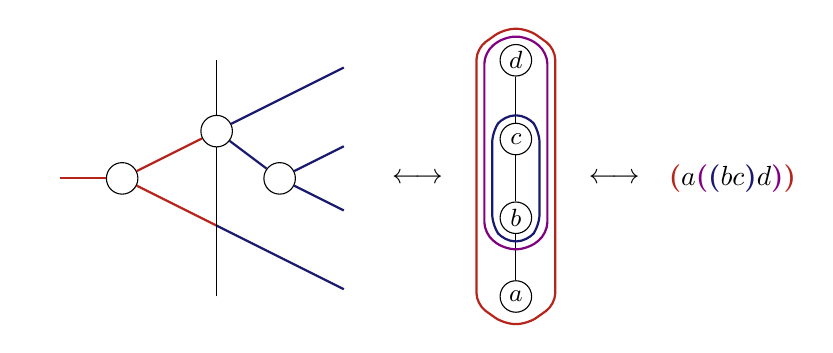
\begin{tikzpicture}

\node (b1)[circle,draw=none,minimum size=4mm,inner sep=0.1mm] at (-2,3) {};
\node (b2)[circle,draw=none,minimum size=4mm,inner sep=0.1mm] at (-2,2) {};
\node (b3) [circle,draw=none,minimum size=4mm,inner sep=0.1mm] at (-2,1) {};
\node (b4) [circle,draw=none,minimum size=4mm,inner sep=0.1mm] at (-2,0) {};
\node (b5) [circle,draw=none,minimum size=4mm,inner sep=0.1mm] at (-6,1.5) {};   


\node (c2) [circle,draw=black,minimum size=4mm,inner sep=0.1mm] at (-3,1.5) {}; 
\node (c1) [circle,draw=black,minimum size=4mm,inner sep=0.1mm] at (-3.8,2.1) {}; 
\node (c3) [circle,draw=black,minimum size=4mm,inner sep=0.1mm] at (-5,1.5) {}; 

\draw[MidnightBlue,thick] (b1)--(c1) node {};
\draw[MidnightBlue,thick] (b2)--(c2) node {};
\draw[MidnightBlue,thick] (b3)--(c2) node {};
\draw[MidnightBlue,thick] (c2)--(c1) node {};

\draw[BrickRed,thick] (c3)--(c1) node {};
\draw[BrickRed,thick] (c3)--(b5) node {};

\draw[BrickRed,thick] (c3)--(-3.8,0.9) node {};
\draw[MidnightBlue,thick] (b4)--(-3.8,0.9) node {};


\draw[-] (-3.8,3)--(c1) node {};
\draw[-] (-3.8,0)--(c1) node {};

\node (B) at (-1.25,1.5) {$\longleftrightarrow$};

\node (x1) [circle,draw=none,minimum size=4mm,inner sep=0.1mm] at (0.15,2.55) {};
\node (x2) [circle,draw=none,minimum size=4mm,inner sep=0.1mm] at (0.15,1.5) {};
\node (x3) [circle,draw=none,minimum size=4mm,inner sep=0.1mm] at (0.15,0.38) {};

\node (t4)[circle,draw=black,minimum size=4mm,inner sep=0.1mm] at (-0,0) {\small $a$};
\node (t3)[circle,draw=black,minimum size=4mm,inner sep=0.1mm] at (0,1) {\small $b$};
\node (t2) [circle,draw=black,minimum size=4mm,inner sep=0.1mm] at (0,2) {\small $c$};
\node (t1) [circle,draw=black,minimum size=4mm,inner sep=0.1mm] at (0,3) {\small $d$};  


\draw[-] (t4)--(t3) node {};
\draw[-] (t3)--(t2) node {};
\draw[-] (t2)--(t1) node {};


\draw [MidnightBlue,rounded corners,thick] (-0.15,0.7) -- (-0.3,0.9) -- (-0.3,2.1) -- (-0.15,2.3) -- (.15,2.3) -- (.3,2.1) -- (.3,.9) -- (.15,.7) -- cycle;
\draw [Purple,rounded corners,thick] (-0.15,0.6) -- (-0.4,0.8) -- (-0.4,3.1) -- (-0.15,3.3) -- (.15,3.3) -- (0.4,3.1) -- (.4,.8) -- (.15,.6) -- cycle;
\draw [BrickRed,rounded corners,thick] (-0.15,-0.35) -- (-0.5,-0.1) -- (-0.5,3.15) -- (-0.15,3.4) -- (.15,3.4) -- (0.5,3.15) -- (0.5,-0.1) -- (0.15,-0.35) -- cycle;


\node (C) at (1.25,1.5) {$\longleftrightarrow$};

\node (D) at (2.75,1.5) {$\red{a \purple{\blue{bc} d}}$};

\end{tikzpicture}}
\caption{Bijections between 2-colored trees, 2-colored nested linear graphs, and 2-colored parenthesizations.}
\label{fig:bijections}
\end{figure}
\end{lemma}

\begin{proof}
This is a simple generalization of the bijection between planar trees and nested linear graphs, see \cref{fig:bijections}. 
Under this bijection, vertices of 2-colored trees correspond to nests, and their colors agree under the previous conventions. 
Also, 2-colored maximal trees are in bijection with maximal 2-colored nested linear graphs. 
\end{proof}

\begin{definition}
We denote by 
\begin{itemize}
  \item $B(\mathcal{N})$ the set of blue nests of the nesting $\mathcal{N}$, and by
  \item $R(\mathcal{N})$ the set of all distinct \emph{unions} of red and purple nests of the nesting $\mathcal{N}$.
\end{itemize}
\end{definition}

To each nest $B \in B(\mathcal{N})$ and to each union of nests $R \in R(\mathcal{N})$, we can associate their \emph{characteristic vectors} $\vec B$ and $\vec R$ which have a $1$ in position $i$ if $i \in B$ (resp. if $i \in \vec R$) and $0$ otherwise.  

\begin{lemma} 
\label{lemma:normalcones}
The normal cone of a face $\mathcal{N}$ of the Ardila--Doker realization of the multiplihedron is given by \[\cone\left(\{-\vec B\}_{B \in B(\mathcal{N})} \cup \{-\vec R\}_{R \in R(\mathcal{N})}\right) \ . \]
\end{lemma}

\begin{proof} 
This follows from the description of the Ardila--Doker multiplihedron as a generalized permutahedron. 
The normal cone of a face of the former is a union of normal cones of faces of the latter. 
These can be easily determined from the projection from the permutahedron to the multiplihedron, written down explicitly in the proof of \cite[Theorem 3.3.6]{Doker11}.
\end{proof}

We are now ready to apply \cref{thm:universalformula} to the multiplihedra. We define \[ D(n)\coloneqq \{(I,J) \ | \ I,J\subset\{1,\ldots,n\}, |I|=|J|, I\cap J=\emptyset, \min(I\cup J)\in I \}. \]

\begin{theorem}
\label{thm:formuladiagonal}
Let $\J_n$ be the Forcey--Loday realization of the multiplihedron, and let $\vec v \in \RR^n$ be a good orientation vector. The cellular image of the diagonal map $\triangle_n : \J_n \to \J_n \times \J_n$ admits the following description: for $\mathcal{N}$ and $\mathcal{N}'$ two 2-colored nestings of the linear graph with $n$ vertices, we have
\begin{eqnarray*}
  (\mathcal{N},\mathcal{N}') \in \Ima\triangle_n 
  & \iff & \forall (I,J) \in D(n), \\
  && \exists B \in B(\mathcal{N}), |B\cap I|>|B\cap J| \text{ or } \\
  && \exists R \in R(\mathcal{N}), |(R\cup \{n\}) \cap I|>| (R\cup \{n\}) \cap J| \text{ or } \\
  && \exists B' \in B(\mathcal{N}'), |B'\cap I|<|B'\cap J| \text{ or } \\
  && \exists R' \in R(\mathcal{N}'), |(R'\cup \{n\}) \cap I|<| (R'\cup \{n\}) \cap J| \ . \\
\end{eqnarray*}
\end{theorem}

\begin{proof} 
The essential ingredient is the computation of the fundamental hyperplane arrangement of the permutahedron, which was already done in \cite[Section 3.1]{LA21}. The result follows in four steps:
\begin{enumerate}
\item Since a good orientation vector $\vec v$ is also a principal orientation vector \cite[Definition 3.15]{LA21}, it orients positively the permutahedron. 
\item \cref{thm:universalformula} then gives a combinatoial description of the cellular image of the diagonal of the permutahedron induced by $\vec v$, which is precisely \cite[Theorem 3.16]{LA21}. 
\item Using \cref{prop:refinementofnormalfans} and the description of the normal cones of the faces of the multiplihedron in \cref{lemma:normalcones}, we get the above formula for the Ardila--Doker realizations of the multiplihedra. 
\item \cref{prop:goodprojection} garantees that this formula holds for the Forcey--Loday realizations, which completes the proof.
\end{enumerate}
\end{proof}

The cellular image of $\triangle_n$ can be represented on $\J_n$ as follows: for each pair of faces $(F,G) \in \Ima \triangle_n$, draw the polytope $(F+G)/2$. 
This defines a polytopal subdivision of $\J_n$.
The polytopal subdivision of $\J_4$ is illustrated on the first page of this article.

\medskip

Let us make this formula explicit in low dimensions. 
We write 2-colored nestings of a linear graph with $n$ vertices as 2-colored parenthesizations of a word with $n$ letters, which are easier to read, see \cref{fig:bijections}. 
We show only pairs of faces $(F,G)$ such that $\dim F + \dim G = \dim P$; the other pairs can be deduced by taking faces.

\begin{equation*}
  \begin{matrix}
      \triangle_2(\purple{ab}) & = & \blue{ab} \times \purple{ab} \cup \purple{ab} \times \red{ab}
  \end{matrix}
\end{equation*}

\begin{equation*}
  \renewcommand*{\arraystretch}{1.5}
  \begin{matrix}
      \triangle_3(\purple{abc}) 
      & = & \blue{\blue{ab} c} \times \purple{abc} 
      & \cup & \purple{abc} \times \red{a \red{bc}}
      & \cup & \blue{abc} \times \purple{a \blue{bc}} \\
      & \cup & \blue{abc} \times \red{a \purple{bc}}  
      & \cup & \purple{a \blue{bc}} \times \red{a \purple{bc}} 
      & \cup & \purple{\blue{ab} c} \times \red{\purple{ab} c} \\
      & \cup & \purple{\blue{ab} c} \times \red{abc} 
      & \cup & \red{\purple{ab} c} \times \red{abc} 
  \end{matrix}
\end{equation*}

\begin{equation*}
  \renewcommand*{\arraystretch}{1.5}
  \begin{matrix}
      & & & & \triangle_4(\purple{abcd}) =  \\
      &  & \blue{\blue{\blue{ab}c}d} \times \purple{abcd} 
      & \cup & \purple{abcd} \times \red{a\red{b\red{cd}}}
      & \cup & \blue{\blue{abc}d} \times \purple{a\blue{bc}d} \\ 
      & \cup & \red{\purple{ab}\purple{cd}} \times \red{ab\red{cd}} 
      & \cup & \blue{\blue{abc}d} \times \purple{a\blue{bcd}} 
      & \cup & \red{\purple{ab}cd} \times \red{ab\red{cd}} \\
      & \cup & \blue{a\blue{bc}d} \times \purple{a\blue{bcd}} 
      & \cup & \red{\purple{abc}d} \times \red{a\red{bc}d}
      & \cup & \blue{\blue{ab}cd} \times \purple{ab\blue{cd}} \\
      & \cup & \red{\purple{abc}d} \times \red{a\red{bcd}} %10
      & \cup & \purple{\blue{\blue{ab}c}d} \times \red{\purple{abc}d}
      & \cup & \purple{ab\blue{cd}} \times \red{a\red{b\purple{cd}}} \\
      & \cup & \purple{\blue{ab}\blue{cd}} \times \red{\purple{ab}\purple{cd}}
      & \cup & \purple{a\blue{bc}d} \times \red{a\red{\purple{bc}d}}
      & \cup & \blue{\blue{ab}cd} \times \red{\purple{ab}\purple{cd}} \\
      & \cup & \purple{a\blue{bc}d} \times \red{a\red{bcd}}
      & \cup & \purple{a\blue{\blue{bc}d}} \times \red{a\purple{bcd}} 
      & \cup & \purple{\blue{ab}cd} \times \red{\purple{ab}\red{cd}}\\
      & \cup & \blue{a\blue{bc}d} \times \red{a\purple{bcd}}
      & \cup & \blue{\blue{abc}d} \times \red{a\purple{bcd}}
      & \cup & \purple{\blue{ab}cd} \times \red{ab\red{cd}} \\
      & \cup & \red{\purple{\blue{ab}c}d} \times \red{\purple{ab}cd}
      & \cup & \purple{a\blue{bcd}} \times \red{a\purple{b\blue{cd}}}
      & \cup & \purple{\blue{\blue{ab}c}d} \times \red{\purple{ab}cd} \\
      & \cup & \purple{a\blue{bcd}} \times \red{a\red{b\purple{cd}}} 
      & \cup & \red{a\purple{bc}d} \times \red{a\red{bcd}}
      & \cup & \red{\red{\purple{ab}c}d} \times \red{abcd} \\
      & \cup & \blue{abcd} \times \purple{a\blue{b\blue{cd}}} 
      & \cup & \red{\purple{\blue{ab}c}d} \times \red{abcd} 
      & \cup & \blue{abcd} \times \red{a\purple{b\blue{cd}}} \\
      & \cup & \purple{\blue{\blue{ab}c}d} \times \red{abcd} 
      & \cup & \blue{abcd} \times \red{a\red{b\purple{cd}}} 
      & \cup & \red{\purple{ab}\blue{cd}} \times \red{ab\purple{cd}} \\
      & \cup & \purple{\blue{abc}d} \times \red{\purple{a\blue{bc}}d}
      & \cup & \purple{\blue{ab}\blue{cd}} \times \red{ab\purple{cd}}
      & \cup & \purple{\blue{abc}d} \times \red{a\red{\purple{bc}d}} \\ %topbot
      & \cup & \purple{\blue{abc}d} \times \red{a\blue{bc}d} %topbot
      & \cup & \blue{\blue{ab}cd} \times \red{ab\purple{cd}}
      & \cup & \purple{\blue{abc}d} \times \red{a\red{bcd}} \\
      & \cup & \red{\purple{a\blue{bc}}d} \times \red{a\purple{bc}d}
      & \cup & \red{\blue{abc}d} \times \red{a\purple{bc}d}  %topbot
      & \cup & \purple{\blue{\blue{ab}c}d} \times \red{a\purple{bc}d} %topbot
  \end{matrix}
\end{equation*}


\medskip

The number of pairs of faces of complementary dimensions in the image of $\triangle_n$ are given, for $n=0$ to $6$, by $1,2,8,42,254,1678$ and $11 790$, respectively. This sequence of integers does not (yet) appear on the Online Encyclopedia of Integer Sequences (OEIS). 

\medskip

For every face $F$ of the multiplihedron $\J_n$, a good orientation vector $\vec v$ defines a unique vertex $\tp F$ (resp. $\bm F$) which maximizes (resp. minimizes) the scalar product $\langle - , \vec v \rangle$. 
By \cite[Proposition 1.15]{LA21}, we have that any pair of faces $(F,G) \in \Ima \triangle_n$ satisfies $\tp F\leq \bm G$. 
In the cases of the simplices, the cubes and the associahedra, the converse also holds: we can characterize the diagonal with a formula of the form $(F,G) \in \Ima \triangle_n \iff \tp F\leq \bm G$.
However, it was shown in \cite{LA21} that this doesn't hold anymore for the operahedra, and in particular for the permutahedra.
This property does not hold either in the case of the multiplihedra. 
For instance, in dimension~$3$ the condition $\tp F\leq \bm G$ determines completely all the pairs in $\Ima \triangle_4$ except four of them: $\purple{\blue{abc}d} \times \red{a\red{\purple{bc}d}}$, $\purple{\blue{abc}d} \times \red{a\blue{bc}d}$, $\red{\blue{abc}d} \times \red{a\purple{bc}d}$ and $\purple{\blue{\blue{ab}c}d} \times \red{a\purple{bc}d}$.
In fact, one can see that the condition $\tp F\leq \bm G$ is equivalent to the conditions in \cref{thm:formuladiagonal} for the pairs $(I,J)$ such that $|I|=|J|=1$. 

\begin{remark}
Observe that our choice of diagonal differs from the one of \cite{SaneblidzeUmble04}. 
For instance, the four pairs of faces above are not part of the image of the Saneblidze--Umble diagonal in dimension $3$. 
A way to relate the two constructions would be to find a choice of chambers in the fundamental hyperplane arrangement of the permutahedra (or the multiplihedra) recovering the latter diagonal, see also \cite[Remark~3.18]{LA21}.
\end{remark}

The formula above, even though easily implemented in the computer, is not optimal. For instance, one could use equation (1) in \cite[Theorem 1.23]{LA21} to reduce the number of pairs $(I,J)$ on which the conditions have to be tested. 
One could also compute directly the fundamental hyperplane arrangement of the Ardila--Doker or Forcey--Loday multiplihedron.
It would be desirable to obtain equivalent combinatorial descriptions of $\Ima \triangle_n$, with a view towards possible applications. 
We sketch some of them in the next sections.


%%%%%%%%%%%%%%%%%%%%%%%%%%%%%%%%%%%%%%%%%%%%


\subsection{Application to $\mathrm{A}_\infty$-algebras and $\mathrm{A}_\infty$-categories} 
\label{sec:Ainftycat}

The diagonal of the associahedra gives a tensor product of $\mathrm{A}_\infty$-algebras, and the diagonal of the multiplihedra gives a tensor product of $\mathrm{A}_\infty$-morphisms.
They also define tensor products on the categorical enrichment of these two notions. 

\begin{definition} 
An $\mathrm{A}_\infty$-category $\cat{A}$ consists of 
\begin{itemize}
  \item a set of objects $\mathrm{Ob}(\cat{A})$,
  \item for each pair of objects $X,Y \in \mathrm{Ob}(\cat{A})$, a graded vector space $\cat{A}(X,Y)$, and
  \item for each $n\geq 1$ and each family of objects $X_0,\ldots,X_n \in \mathrm{Ob}(\cat{A})$, a linear map \[m_n : \cat{A}(X_0,X_1) \otimes \cdots \otimes \cat{A}(X_{n-1},X_n) \to \cat{A}(X_0,X_n)\] of degree $|m_n|=n-2$, satisfying the equations \[\sum_{\substack{p+q+r=n \\ 2 \leq q \leq n-1}} (-1)^{p+qr}m_{p+1+r}(\id^{\otimes p} \otimes m_q \otimes \id^{\otimes r}) = 0 \ , \ n\geq 1 \ .\]
\end{itemize}
\end{definition}

Observe that an $\mathrm{A}_\infty$-algebra is just an $\mathrm{A}_\infty$-category with one object.
Thus, the diagonal of the associahedra provides us with a canonical 
$\mathrm{A}_\infty$-category structure on the tensor product $\cat{A}\otimes \cat{B}$ of two $\mathrm{A}_\infty$-categories, which we describe now. 

\begin{definition}
Let $(\gra,\mathcal{N})$ be a nested linear graph. The \emph{left-levelwise order} on $\mathcal{N}$ is defined as follows: we order the nests by decreasing cardinality, and we order two nests of same cardinality by comparing their minimal elements. 
\end{definition}
The left-levelwise order on a nesting is induced by the left-levelwise order on trees, under the bijection of \cref{lemma:bijection}.

\begin{definition} 
\label{def:signs}
Let $\gra$ be a linear graph.  
\begin{enumerate}[leftmargin=*]
\item For a nesting $\mathcal{N}$ of $\gra$, we denote by $N_i$ the unique minimal nest of $\mathcal{N}$ containing the edge $i$, with respect to nest inclusion. 
\item An edge $i$ of $\gra$ is \emph{admissible} if $i \neq \min N_i$. We denote the set of admissible edges of $\mathcal{N}$ by $\mathrm{Ad}(\mathcal{N})$. 
\item Given a pair of nestings $\mathcal{N}, \mathcal{N}'$, we give the set $\mathrm{Ad}(\mathcal{N})\sqcup \mathrm{Ad}(\mathcal{N}')$ the total order by using the left-levelwise order on the nestings and within a nest by following the numbering of the edges in increasing order. 
\item The function $\sigma_{\mathcal{N}\mathcal{N}'}: \mathrm{Ad}(\mathcal{N})\sqcup \mathrm{Ad}(\mathcal{N}') \to (1,2,\ldots,|\mathrm{Ad}(\mathcal{N})\sqcup \mathrm{Ad}(\mathcal{N}')|)$ defined on $i \in \mathrm{Ad}(\mathcal{N})$ by 
\begin{equation*}
  \sigma_{\mathcal{N}\mathcal{N}'}(i)= 
  \begin{cases}
    \min N_i -1 & \text{ if } i \in \mathrm{Ad}(\mathcal{N})\cap \mathrm{Ad}(\mathcal{N}') \text{ and } 1 \neq \min N_i < \min N_i' \\ 
    i-1 & \text{ otherwise ,} 
  \end{cases}
\end{equation*}
and similarly on $i \in \mathrm{Ad}(\mathcal{N}')$ by inversing the roles of $\mathcal{N}$ and $\mathcal{N}'$, induces a permutation of the set $\{1,2,\ldots,|\mathrm{Ad}(\mathcal{N})\sqcup \mathrm{Ad}(\mathcal{N}')|\}$ that we still denote by $\sigma_{\mathcal{N}\mathcal{N}'}$.
\end{enumerate}
\end{definition}

We are now ready to define the tensor product of two $\mathrm{A}_\infty$-categories. We denote by $\sigma_n$ the isomorphism $(A_1 \otimes B_1)\otimes (A_2 \otimes B_2) \otimes \cdots \otimes (A_n \otimes B_n) \cong (A_1 \otimes \cdots \otimes A_n) \otimes (B_1 \otimes \cdots \otimes B_n)$. 

\begin{proposition} The \emph{tensor product} $\cat{A}\otimes \cat{B}$ of two $\mathrm{A}_\infty$-categories $\cat{A}$ and $\cat{B}$ is given by 
\begin{itemize}
  \item the set of objects $\mathrm{Ob}(\cat{A}\otimes \cat{B})\coloneqq \mathrm{Ob}(\cat{A})\times\mathrm{Ob}(\cat{B})$,
  \item for each pair of objects $X_1\times Y_1,X_2\times Y_2 \in \mathrm{Ob}(\cat{A}\otimes \cat{B})$, the space of morphisms $\cat{A}\otimes \cat{B}(X_1\times Y_1,X_2\times Y_2)\coloneqq \cat{A}(X_1,X_2)\otimes\cat{B}(Y_1,Y_2)$,
  \item for each $n\geq 1$ and each family of objects $X_0\times Y_0,\ldots,X_n\times Y_n \in \mathrm{Ob}(\cat{A}\otimes \cat{B})$, the linear map 
  \begin{equation*}
  \rho_n : \cat{A}\otimes \cat{B}(X_0\times Y_0,X_1\times Y_1) \otimes  \cdots  \otimes \cat{A}\otimes \cat{B}(X_{n-1}\times Y_{n-1},X_n\times Y_n) \\ 
   \to \cat{A}\otimes \cat{B}(X_0\times Y_0,X_n\times Y_n) 
\end{equation*} 
defined by 
\[\rho_n \coloneqq 
\sum_{\substack{
  \mathcal{N},\mathcal{N}' \in \mathcal{N}(\gra) \\ 
  |\mathcal{N}|+|\mathcal{N}'|=|V(\gra)| \\
  \forall i<j, \exists N \in \mathcal{N}, i \in \mathcal{N} \text{ and } j \notin \mathcal{N} \text{ or } \\
  \exists N' \in \mathcal{N}', i \notin \mathcal{N} \text{ and } j \in \mathcal{N}'
}}
(-1)^{|\mathrm{Ad}(\mathcal{N})\cap \mathrm{Ad}(\mathcal{N}')|}\mathrm{sgn}(\sigma_{\mathcal{N}\mathcal{N}'})\mathcal{N}(m_n)\otimes \mathcal{N}'(m_n') \ \sigma_n \ ,\] 
where $\gra$ is a linear graph, and where $\mathcal{N}(m_n)$ and $\mathcal{N}'(m_n')$ denote the composition of the structural maps $\{m_n\}$ and $\{m_n'\}$ of $\cat{A}$ and $\cat{B}$ respectively, corresponding to the nests of $\mathcal{N}$ and $\mathcal{N}'$ in the left-levelwise order.
\end{itemize}
\end{proposition}

\begin{proof}
  The formula for the $\rho_n$'s stems from our choice of diagonal on the associahedra; the fact that they satisfy the $\mathrm{A}_\infty$ relations follows from the construction and the functoriality in \cref{prop:functoriality}. The signs depend on our choice of cellular orientations on the associahedra, and they are obtained via the computation of a determinant. We refer to the proof of \cite[Proposition 4.27]{LA21} for more details. 
\end{proof}

Now we treat the case of $\mathrm{A}_\infty$-functors between $\mathrm{A}_\infty$-categories. 

\begin{definition}
An $\mathrm{A}_\infty$-functor $f : \cat{A} \rightsquigarrow \cat{B}$ between two $\mathrm{A}_\infty$-categories consists of 
\begin{itemize}
\item a function $\mathrm{Ob}(f) : \mathrm{Ob}(\cat{A}) \to \mathrm{Ob}(\cat{B})$,
\item for each $n \geq 1$ and each family of objects $X_0, \ldots, X_n \in \mathrm{Ob}(\cat{A})$, a linear map \[f_n : \cat{A}(X_0,X_1) \otimes \cdots \otimes \cat{A}(X_{n-1},X_n) \to \cat{B}(f(X_0),f(X_n))\] of degree $|f_n|=n-1$, satisfying the equations \[
  \sum_{\substack{i_1+\cdots+i_k=n \\ k \geq 1}} (-1)^{\varepsilon} m_k'(f_{i_1}\otimes\cdots\otimes f_{i_k}) = 
  \sum_{\substack{p+q+r=n \\ 2 \leq q \leq n-1}} (-1)^{p+qr}f_{p+1+r}(\id^{\otimes p} \otimes m_q \otimes \id^{\otimes r}) = 0 \ , \ n\geq 1 \ ,\] where $\varepsilon = \sum_{u=1}^{k}(k-u)(1-i_u)$.
\end{itemize}
\end{definition}

Observe that an $\mathrm{A}_\infty$-functor between two $\mathrm{A}_\infty$-categories with one object is just an $\mathrm{A}_\infty$-morphism between two $\mathrm{A}_\infty$-algebras.
Thus, the diagonal of the multiplihedra provides us with a canonical $\mathrm{A}_\infty$-functor structure from $\cat{A}\otimes \cat{B}$ to $\cat{A}'\otimes \cat{B}'$ associated to two $\mathrm{A}_\infty$-functors $\cat{A}\rightsquigarrow \cat{A}'$ and $\cat{B} \rightsquigarrow \cat{B}'$~. 

\begin{definition} For 2-colored nestings $\mathcal{N}$ and $\mathcal{N}'$, we use the same definitions as in \cref{def:signs}, but with the following two modifications:
\begin{enumerate}[leftmargin=*]
\item[(2)] We say that an edge $i$ of $g$ is \emph{admissible} when $N_i$ is bicolored, or if $i \neq \min N_i$ when $N_i$ is monochrome. 
\item[(4)] The function $\sigma_{\mathcal{N}\mathcal{N}'}: \mathrm{Ad}(\mathcal{N})\sqcup \mathrm{Ad}(\mathcal{N}') \to (1,2,\ldots,|\mathrm{Ad}(\mathcal{N})\sqcup \mathrm{Ad}(\mathcal{N}')|)$ is defined on $i \in \mathrm{Ad}(\mathcal{N})$ by 
\begin{equation*}
  \sigma_{\mathcal{N}\mathcal{N}'}(i)= 
  \begin{cases}
    \min N_i & \text{ if } i \in \mathrm{Ad}(\mathcal{N})\cap \mathrm{Ad}(\mathcal{N}') , N_i \text{ is monochrome and } N_i' \text{ is not} \\
    \min N_i & \text{ if } i \in \mathrm{Ad}(\mathcal{N})\cap \mathrm{Ad}(\mathcal{N}'), N_i \text{ and } N_i' \text{ are monochrome and } \min N_i < \min N_i' \\ 
    i & \text{ otherwise ,} 
  \end{cases}
\end{equation*}
and similarly on $i \in \mathrm{Ad}(\mathcal{N}')$ by inversing the roles of $\mathcal{N}$ and $\mathcal{N}'$.
\end{enumerate}
\end{definition}

For convenience, let us recall that \[ D(n)\coloneqq \{(I,J) \ | \ I,J\subset\{1,\ldots,n\}, |I|=|J|, I\cap J=\emptyset, \min(I\cup J)\in I \}. \]
Let us denote by $\text{mono}(\mathcal{N})$ the set of monochrome nests of a nesting $\mathcal{N}$.

\begin{proposition}
The \emph{tensor product} $f\otimes g$ of two $\mathrm{A}_\infty$-functors $f:\cat{A}\rightsquigarrow \cat{A}'$ and $g:\cat{B} \rightsquigarrow \cat{B}'$ is given by 
\begin{itemize}
\item the function $\mathrm{Ob}(f\otimes g)\coloneqq \mathrm{Ob}(f)\times \mathrm{Ob}(g) : \mathrm{Ob}(\cat{A}\otimes\cat{B}) \to \mathrm{Ob}(\cat{A}'\otimes\cat{B}')$,
\item for each $n\geq 1$ and each family of objects $X_0\times Y_0,\ldots,X_n\times Y_n \in \mathrm{Ob}(\cat{A}\otimes\cat{B})$, the linear map 
\begin{eqnarray*}
h_n : (\cat{A}\otimes \cat{B})(X_0\times Y_0,X_1\times Y_1) \otimes  \cdots \otimes (\cat{A}\otimes \cat{B})(X_{n-1}\times Y_{n-1},X_n\times Y_n) \\
\to (\cat{A}'\otimes \cat{B}')(f(X_0)\times g(Y_0),f(X_n)\times g(Y_n)) 
\end{eqnarray*}
defined by 
\[h_n \coloneqq 
\sum_{\substack{
\mathcal{N},\mathcal{N}' \in \mathcal{N}_2(\gra), \ |\text{mono}(\mathcal{N})|+|\text{mono}(\mathcal{N}')|=|E(\gra)| \\
\forall (I,J) \in D(n), \exists B \in B(\mathcal{N}), |B\cap I|>|B\cap J| \text{ or } \\
\exists R \in R(\mathcal{N}), |(R\cup \{n\}) \cap I|>| (R\cup \{n\}) \cap J| \text{ or } \\
\exists B' \in B(\mathcal{N}'), |B'\cap I|<|B'\cap J| \text{ or } \\
\exists R' \in R(\mathcal{N}'), |(R'\cup \{n\}) \cap I|<| (R'\cup \{n\}) \cap J| 
 }} 
(-1)^{|\mathrm{Ad}(\mathcal{N})\cap \mathrm{Ad}(\mathcal{N}')|}
\mathrm{sgn}(\sigma_{\mathcal{N}\mathcal{N}'})
\mathcal{N}(f)\otimes \mathcal{N}'(g) \ \sigma_n \ ,\]
where $\gra$ is a linear graph, and where $\mathcal{N}(f)$ and $\mathcal{N}'(g)$ denote the composition of the structural maps $\{f_n\}$ and $\{g_n\}$ corresponding to the nests of $\mathcal{N}$ and $\mathcal{N}'$ in the left-levelwise order.
\end{itemize}
\end{proposition}


\begin{proof}
  The formula for the $h_n$'s stems from our choice of diagonal on the multiplihedra; the fact that they satisfy the $\mathrm{A}_\infty$ relations follows from the construction and the functoriality in \cref{prop:functoriality}. The signs depend on our choice of cellular orientations on the multiplihedra, and they are obtained via the computation of a determinant. We refer to \cite[Section 4.3]{LA21} for more details. 
\end{proof}

%%%%%%%%%%%%%%%%%%%%%%%%%%%%%%%%%%%%%%%%%%%%%%%

\subsection{Further directions} \label{sec:furtherdirections}

\subsubsection{Monoidality}
The tensor products defined above do not make the category of $\mathrm{A}_\infty$-categories with $\mathrm{A}_\infty$-functors into a monoidal category, in the strict sense of the term. There are two obstructions to this:
\begin{enumerate}
  \item The diagonal maps $\K_n \to \K_n \times \K_n$ and $\J_n \to \J_n \times \J_n$ are not cellularly coassociative, hence under the cellular chains functor, they do not define associative tensor products. 
  According to a result of M. Markl and S. Schnider \cite[Section 6]{MarklShnider06}, such an associative tensor product does not exist.
  \item The tensor product above is not compatibile with the composition of $\mathrm{A}_\infty$-morphisms \Guillaume{[...] Counterexample!}. 
  We belive that there is a way to prove, in a similar fashion to the preceding point, that such a functorial tensor product cannot exist.
\end{enumerate}

$\mathtt{\Ainf -alg}$

\subsubsection{Applications in symplectic topology}
There are three main applications:
\begin{enumerate}
  \item Armorim \Guillaume{TBC}
  \item The above functorial tensor product can be used in symplectic topology to relate the Fukaya category of a product of symplectic manifold to the product of the Fuakaya categories of the manifolds. \Guillaume{TBC}
  \item LOT; The definition of the above tensor product by an explicit formula that can be easily implemented on the computer, and could be applied to calculate explicitely invariants of 4-dimensonal symplectic manifolds. For instance, R. Lipshitz, P. Osv\'ath and D. P. Thurston define in \cite{LOT20} diagonals of the multiplihedra to study bordered Floer homology of ... These invariants detect exotic smooth structures ... \Guillaume{TBC}
\end{enumerate}


\bibliographystyle{amsalpha}
\bibliography{bib}

%\bigskip
%\hrule
%\bigskip

%\newpage

%\begin{align*}
%& La\TreeLa \\
%& Lb\TreeLb \\
%& Lc\TreeLc \\
%& Ra\TreeRa \\
%& Rb\TreeRb \\
%& Rc\TreeRc \\
%& Lab\TreeLab \\
%& Rab\TreeRab \\
%& Lbc\TreeLbc \\
%& Rbc\TreeRbc \\
%& Ca\TreeCa \\
%& Cb\TreeCb \\
%& Cab\TreeCab \\
%& Iab\TreeIab \\
%\end{align*}


%\begin{align*}
%& R\TreeR \\
%& L\TreeL \\
%& LL\TreeLL \\
%& LR\TreeLR \\
%& RR\TreeRR \\
%& RL\TreeRL \\
%& CC\TreeCC \\
%& AL\TreeAL \\
%& RA\TreeRA \\
%& AR\TreeAR \\
%& LA\TreeLA \\
%& CA\TreeCA \\
%& C\TreeC \\
%\end{align*}






\end{document}
